\chapter[Caractérisation d'un modèle d'Intelligence Artificielle]{Caractérisation d'un modèle d'Intelligence Artificielle}

\boitemagique{Dans ce chapitre}{
Ce chapitre propose une méthode de caractérisation globale d'un modèle. L'objectif est de construire une représentation mentale du modèle. Un extrait pertinent de paires d'exemples de contre-exemples proches.
La stratégie puis l'implémentation de la méthode sont présentées. L'application met en avant les avantages et limites de la proposition.
Cette méthode de caractérisation est prometteuse, mais reste à comparer à d'autres méthodes de la littérature.
}

% Avant
Nous avons présenté dans les chapitres précédents des explications locales.
Dans ce chapitre, nous caractérisons globalement un modèle d'IA.
Ce chapitre répond à des besoins d'auditabilité et des contraintes légales.
% Objectif
Notre objectif est de permettre aux utilisateurs de créer un modèle mental fidèle au modèle caractérisé. La notion de \textit{modèle mental} est introduite en section~\ref{C1:generation}.
% comment
Nous proposons une méthodologie générale de caractérisation, qui s'appuie sur les limites de décision par classe d'un modèle d'IA

% Résultats
Nous présentons notre protocole et l'appliquons à un cas d'utilisation réel dans le domaine du traitement du langage naturel.
L'application montre son potentiel sur l'une des classes d'un modèle de classification. L'analyse de l'explication permet d'appréhender des éléments clés de la frontière de décision, et d'émettre des hypothèses d'amélioration du jeu de données d'entraînement.
Nous notons également des marges d'amélioration. Ainsi l'ajout d'une méthode d'explication locale est nécessaire pour l'analyse des textes longs.

% plan
Nous présentons en section~\ref{C4:strategie} la méthode de caractérisation, et son implémentation en section~\ref{C4:implémentation}. Enfin, nous appliquons cette caractérisation en section~\ref{C4:application}.



\section{Stratégie}  \label{C4:strategie}
%  quel type d'explication, quel besoin, dans quel contexte, quelle méthode pour y répondre
Nous nous  intéressons au contexte de la classification multi-label, multi-classes.
Dans le chapitre~\ref{C1}, nous présentons Lime, méthode d'explication locale, et son explication globale associée : SP-Lime~\cite{Ribeiro2016}. Cette explication globale s'appuie sur des exemples dont l'explication Lime a été réalisée au préalable. Elle est donc coûteuse. Toutefois, c'est cette philosophie qui conduit la suite des travaux présentés dans ce chapitre.

% Afin de permettre à l'utilisateur de créer son modèle mental, le modèle est décrit classe par classe.
Comment permettre à l'utilisateur d'avoir un modèle mental fidèle au comportement réel du modèle original (MO) ? Pour résoudre cette problématique, nous proposons d'aider à l'appréhension des frontières de décision du MO. Cette aide se traduit par l'analyse d'un ensemble limité d'exemples et de contre-exemples pour une classe donnée, comme illustré avec le tableau~\ref{tab:illus_e_cfe}. Un exemple, dans la première colonne du tableau, correspond ici à la classe étudiée et un contre-exemple, dans la seconde colonne, est un élément d'une autre classe. L'ensemble des couples d'exemple et contre-exemple permet d'appréhender différents aspects d'une classe, notamment ses frontières avec d'autres classes. Les exemples situés au c\oe ur d'une classe nous semblent moins pertinents.

% Qu'est-ce que je présente à l'utilisateur ?
\begin{table}[htpb!]
    \caption{Délimitation de la classe \textit{``Discrimination : Contrat étudiant''}  sous la forme d'exemples et contre-exemples associés} \label{tab:illus_e_cfe}
    \begin{tabular}{|p{0.45\textwidth}|p{0.50\textwidth}|} \hline
    \textbf{Exemple type}                                            & \textbf{Contre-exemple associé}     \\ \hline
    Profil recherché: Etudiant(e), salarié(e), retraité(e). & Etudiant(e), retraité(e), travaillant à temps partiel ou   en recherche d'emploi, vous êtes avant tout passionné(e) par les enfants? \\ \hline
    Etudiants acceptés.                                     & 35 H/Semaine minimum Etudiants acceptés. \\ \hline
    \end{tabular}
\end{table}

Un utilisateur ne peut recevoir un nombre trop important d'éléments à traiter à la fois. Ces exemples doivent donc être habilement sélectionnés. Illustrée en figure~\ref{fig:strategie}, notre stratégie consiste à prendre un ensemble d'exemples candidats, puis de filtrer et trier les exemples qui en sont issus. Le filtre vise à conserver uniquement les exemples qui ont une pertinence technique pour représenter le comportement du MO. Il est possible que le filtre ne suffise pas pour montrer un ensemble restreint d'une dizaine d'éléments à un utilisateur ou une utilisatrice. Un tri est alors effectué avec pour but de proposer un résumé digeste et représentatif pour l'utilisateur. Ce tri peut être laissé à la main de l'utilisateur.

\begin{figure}[h!tpb]
 \centering 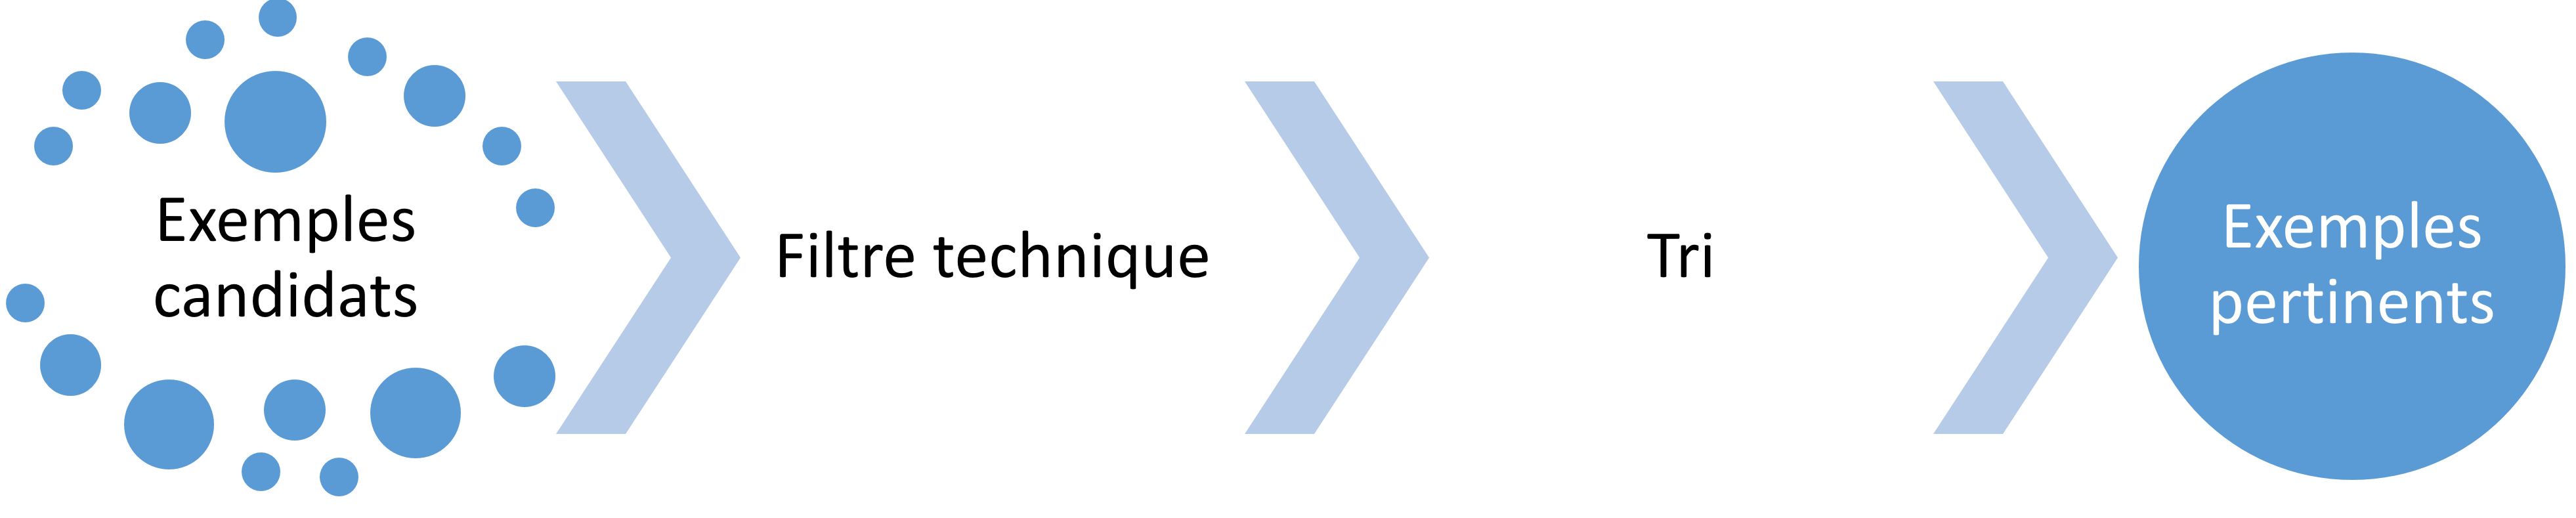
\includegraphics[width=0.9\textwidth]{S4-Explicabilite_globale/figures/strategie.png}
\caption{La stratégie de sélection des exemples à présenter à l'utilisateur.} \label{fig:strategie}
\end{figure}

La figure~\ref{fig:strategie} présente l'enchainement de définition d'exemples candidats, filtre, et tri de ces exemples. Les détails sont volontairement mis de côté, nous proposons une méthodologie générale dont les implémentations des différents éléments sont à adapter.

% Transition
Maintenant que nous avons défini ce que nous souhaitons présenter aux utilisateurs, et la stratégie générale, nous pouvons définir l'implémentation de cette stratégie.

\section{Implémentation} \label{C4:implémentation}

Dans cette section, nous présentons cette implémentation ainsi que nos choix techniques.
Tous les éléments présentés ici sont des choix d'implémentation qui ne sont pas fixés. Il est possible de modifier les trois étages présentés ici, en conservant la structure présentée en section précédente.
Nous proposons cette première solution fonctionnelle, appliquée sur un cas d'usage en section~\ref{C4:application}. Celle-ci reste à évaluer, et adapter à d'autres situations et contraintes.

 Nous présenterons en premier lieu la sélection d'un ensemble d'exemples candidats en section~\ref{C4:candidats}. En section~\ref{C4:filtre} nous détaillerons le filtre technique effectué, et en section~\ref{C4:tri} le tri appliqué.

\subsection{Choix de la source d'exemples candidats} \label{C4:candidats}

Les exemples présentés aux utilisateurs dans la littérature peuvent être issus des données réelles, comme dans~\cite{Ribeiro2016}. Les candidats sont alors les données d'entraînement, de développement et de test. Ces exemples peuvent également être générés. Dans~\cite{Charachon2021}, les auteurs créent des explications sous la forme de la différence entre des exemples et contre-exemples générés. Les techniques de génération actuelles permettent de créer des données complexes telles que des textes~\cite{Wang2021} et images~\cite{Ramesh2022}.

Générer les exemples et contre-exemples nécessite un apprentissage supplémentaire du modèle générateur, et crée des données non connues par le MO. L'entraînement d'un modèle générateur ajoute une technique d'apprentissage profond. Cette méthode a pour risque de reporter le problème d'explication à ce nouveau modèle générateur. Afin de réduire les efforts des utilisateurs pour reconstruire leur modèle mental, nous nous appuyons sur des exemples candidats concrets.
Nous préférons nous appuyer sur les données issues de la base d'apprentissage, permettant ainsi de ne pas s'appuyer sur une couche supplémentaire d’apprentissage profond. Nous nous assurons aussi d'avoir uniquement des données réelles, nécessitant en contrepartie d'avoir accès au jeu de données d'entraînement.

Toutes les données d'entraînement n'ont pas le même impact sur le comportement du modèle. Comme défini en section~\ref{C4:strategie}, nous souhaitons conserver, parmi les exemples candidats, uniquement ceux qui ont une pertinence du point de vue du MO.

\subsection{Filtre} \label{C4:filtre}

Ces exemples pertinents sont ceux qui représentent le fonctionnement du MO. Nous cherchons notamment les données présentes aux frontières de décision, qui pourraient être récupérées en filtrant les données d'apprentissage qui en sont proches.

% Approche centrée NN
Pour déterminer ces points, différentes approches existent. Nous pouvons par exemple nous appuyer sur le fonctionnement d'un réseau de neurones. Les points dont le score de prédiction (sortie du MO) est proche de 0,5 pour une classe donnée correspondent à des points qui ne sont pas typiques de cette classe. Cependant, il est plus difficile de dire si ces points sont situés près d'une frontière ou s'ils ont un score faible car ils sont hors de la distribution des données ou aberrants.

% Approche sur les données
Il est également possible de prendre des points antagonistes (de classes différentes) proches  d'une manière centrée sur les données.
En définissant une fonction de distance entre les points, nous pouvons sélectionner le couple de points les plus proches qui appartiennent à deux décisions de modèle différentes comme antagonistes. Mais ces points peuvent ne pas être les plus représentatifs de la frontière de décision. Dans un contexte de classification One \textit{vs.} Rest, plusieurs couples d'instances de données peuvent être nécessaires pour bien définir la frontière de décision. Dans un mode One \textit{vs.} One, si deux classes sont éloignées dans l'espace de représentation, le couple d'instances de données résultant n'aura aucun intérêt. Certaines frontières complexes nécessitent également la définition de plus d'un couple d'exemples.

Nous proposons un filtre basé sur les SVM pour extraire les exemples factuels et contrefactuels pertinents. Le filtre s'appuie sur la notion de vecteurs supports du SVM, soit les points de données importantes pour l'apprentissage du SVM. Il est composé de 3 étapes : suppression des doublons, sélection des vecteurs supports et appairage.
% TODO Harold : ajouter un argumentaire :
% - classifieur fortement discriminant permettant de se focaliser sur les frontières
% - se base sur les données d'apprentissage pour la définition du modèle ( les vecteurs supports)
% - utilisation de noyaux gaussiens pour retrouver un pouvoir génératif ( on peut retrouver les données utilisées)
% - un seul paramètres pour choisir le compromis de complexité biais/variance: C
\begin{figure}[h!tpb]
    \begin{subfigure}[t]{0.45\textwidth}
      \centering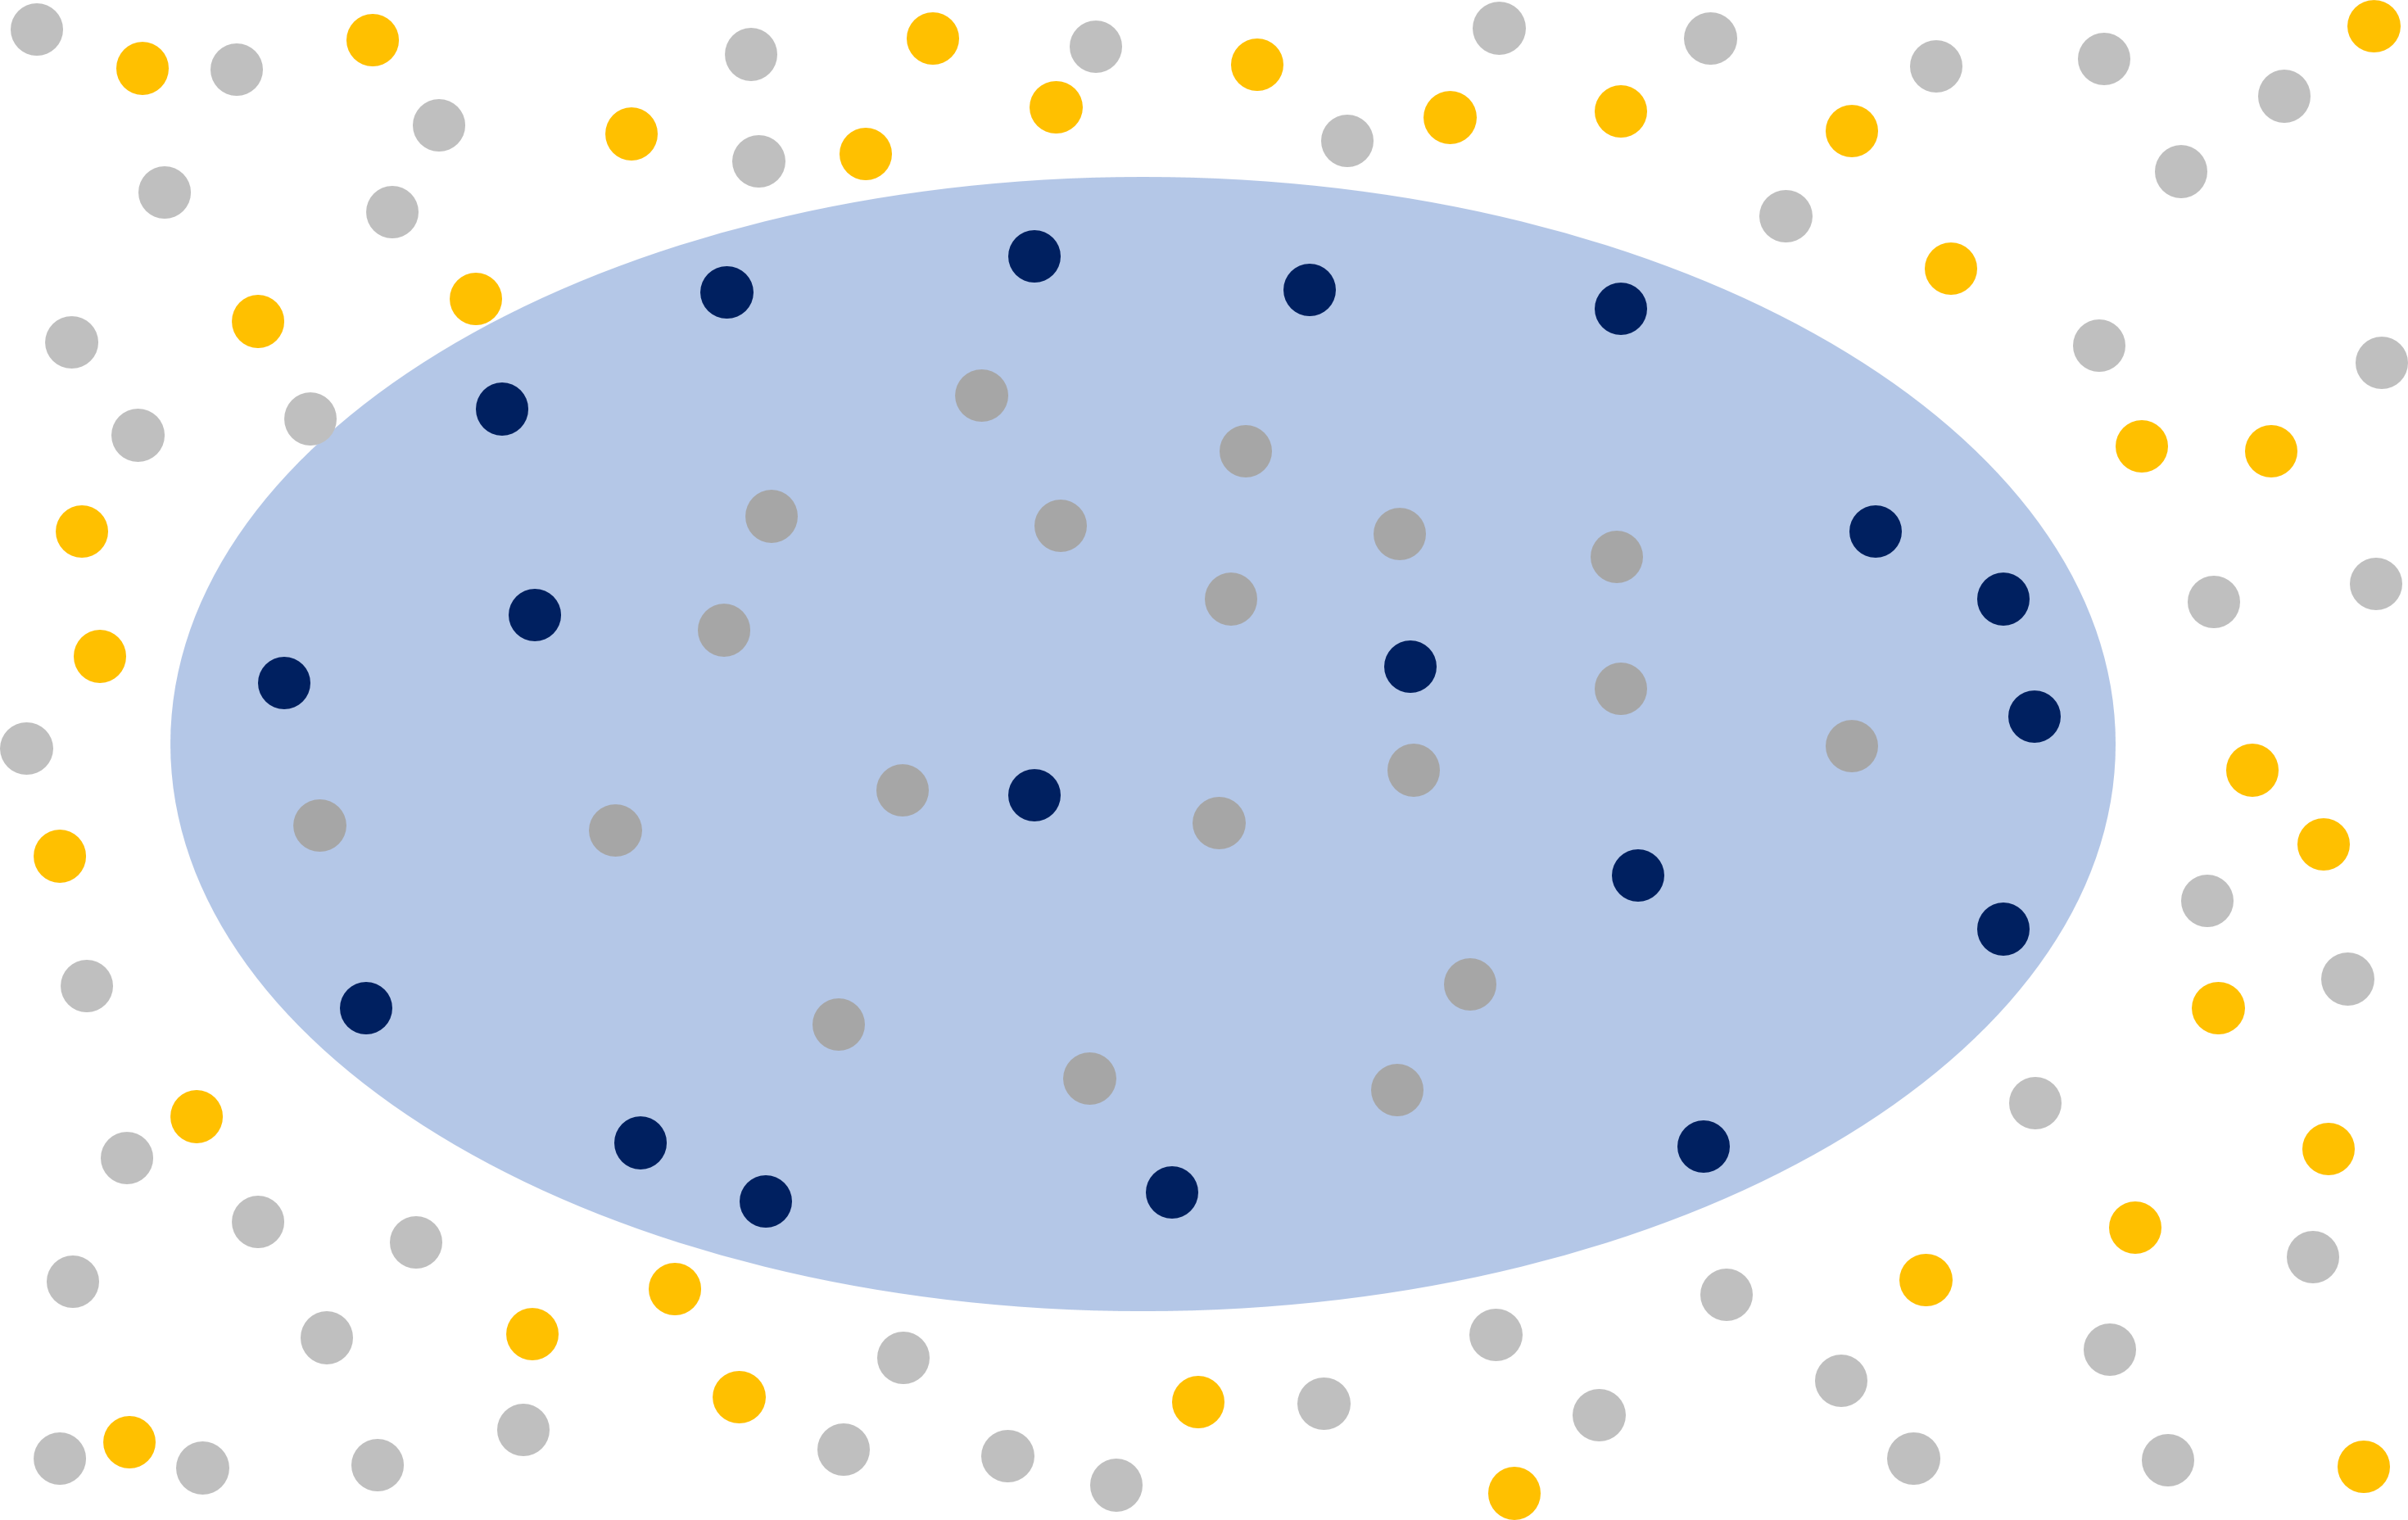
\includegraphics[width=\textwidth]{S4-Explicabilite_globale/figures/filtre1.png}
      \caption{Les données candidates. Les points bleus et jaunes correspondent aux vecteurs supports protagonistes et antagonistes. Les autres points de données sont en gris}  \label{fig:filtre1}
    \end{subfigure} \qquad
    \begin{subfigure}[t]{0.45\textwidth}
      \centering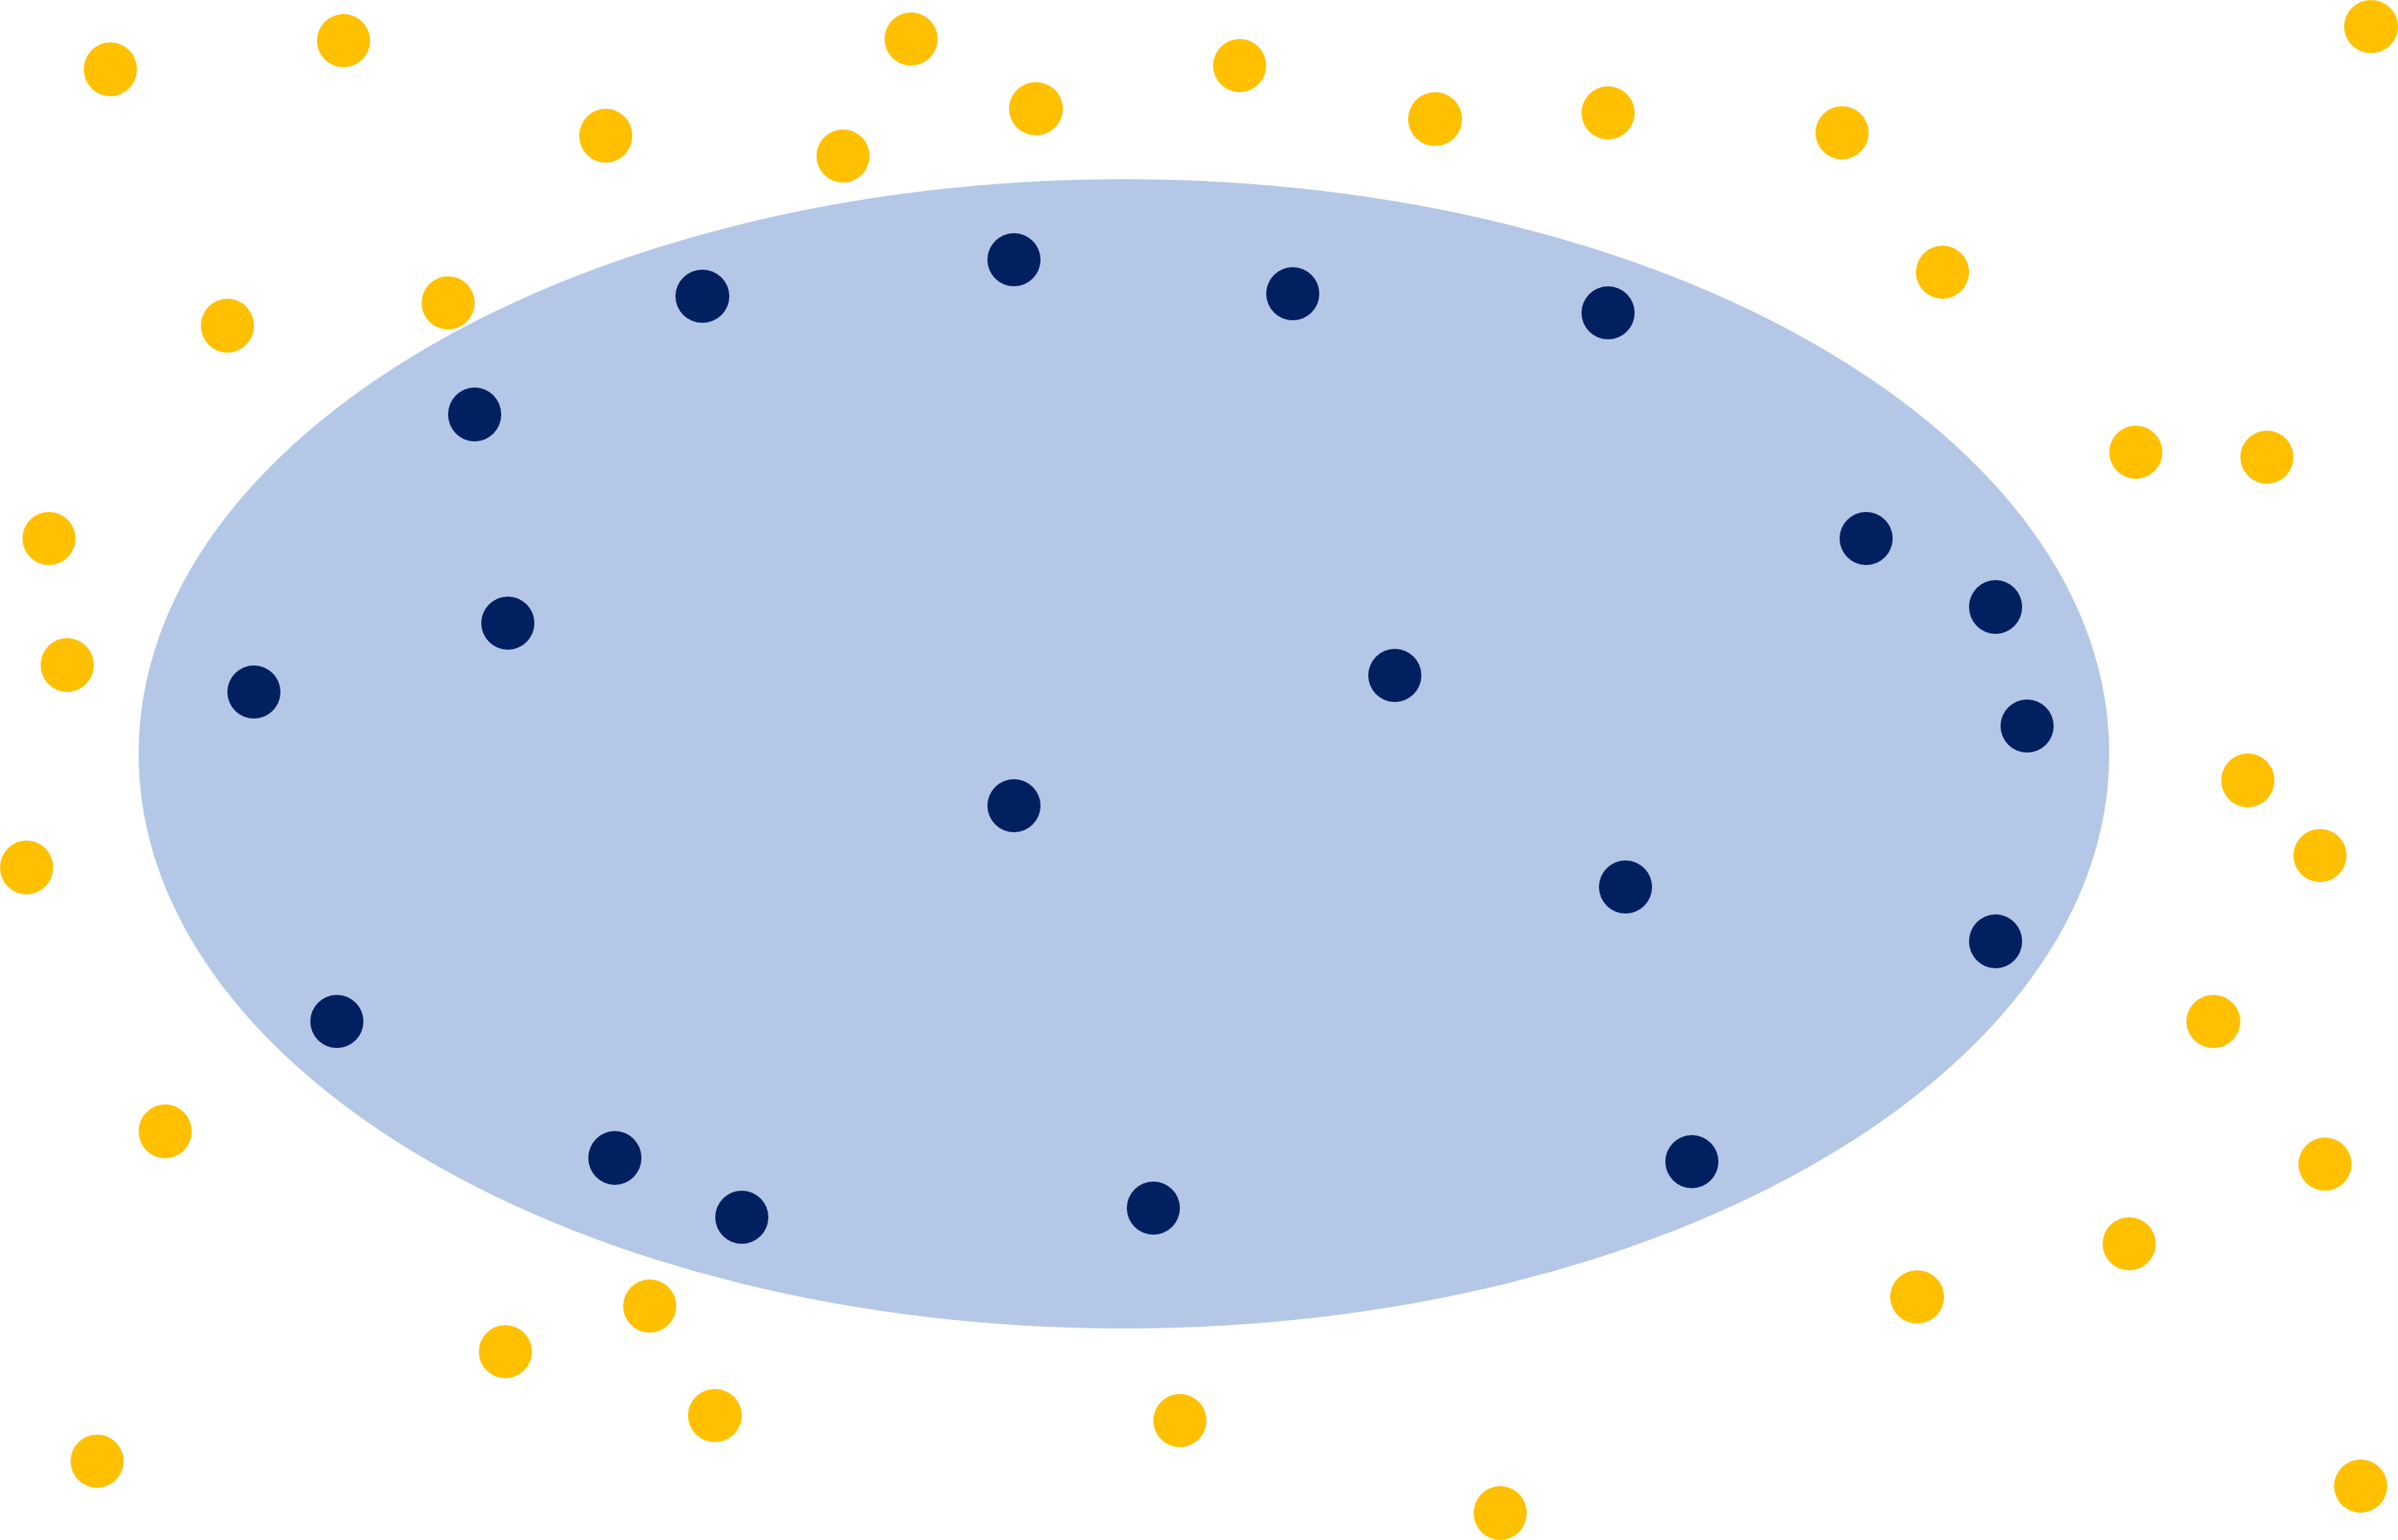
\includegraphics[width=\textwidth]{S4-Explicabilite_globale/figures/filtre2.png}
      \caption{ Les points qui ne sont pas des vecteurs supports sont supprimés.} \label{fig:filtre2}
  \end{subfigure}

    \begin{subfigure}[t]{0.45\textwidth}
      \centering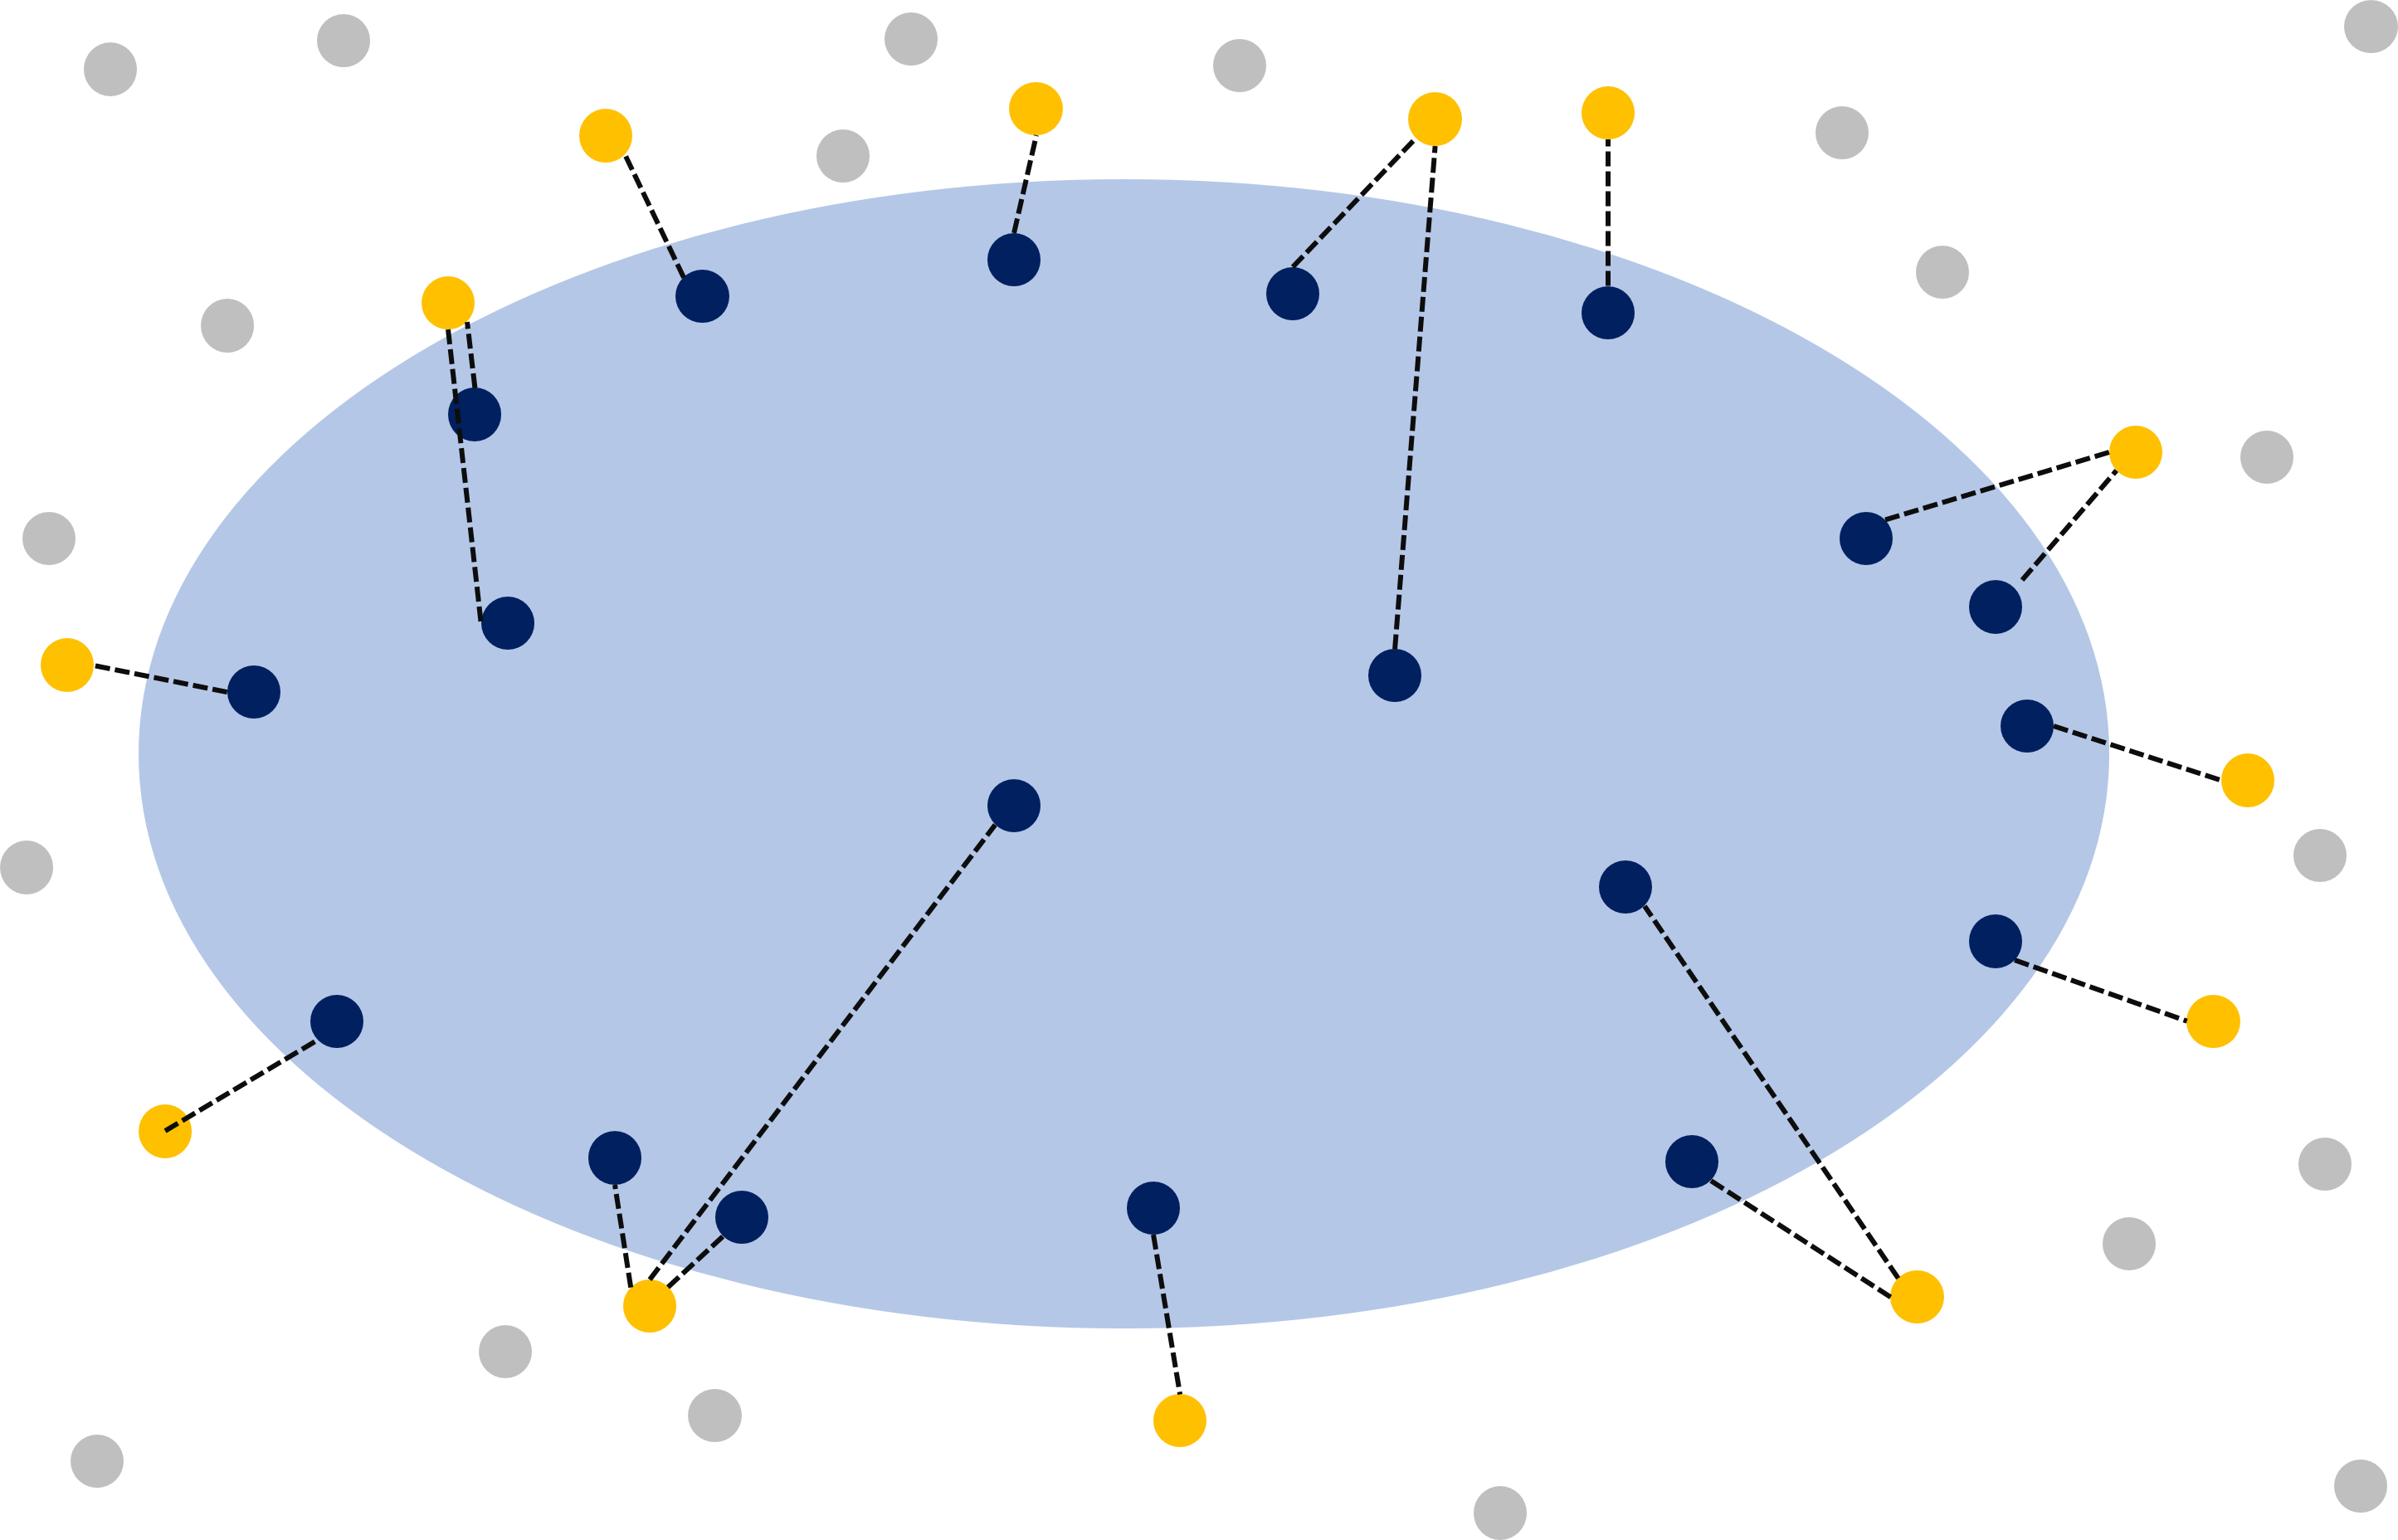
\includegraphics[width=\textwidth]{S4-Explicabilite_globale/figures/filtre3.png}
      \caption{Chaque vecteur support protagoniste est apparié au vecteur support antagoniste le plus proche. Les vecteurs supports antagonistes non appariés sont grisés.} \label{fig:filtre3}
    \end{subfigure} \qquad
    \begin{subfigure}[t]{0.45\textwidth}
      \centering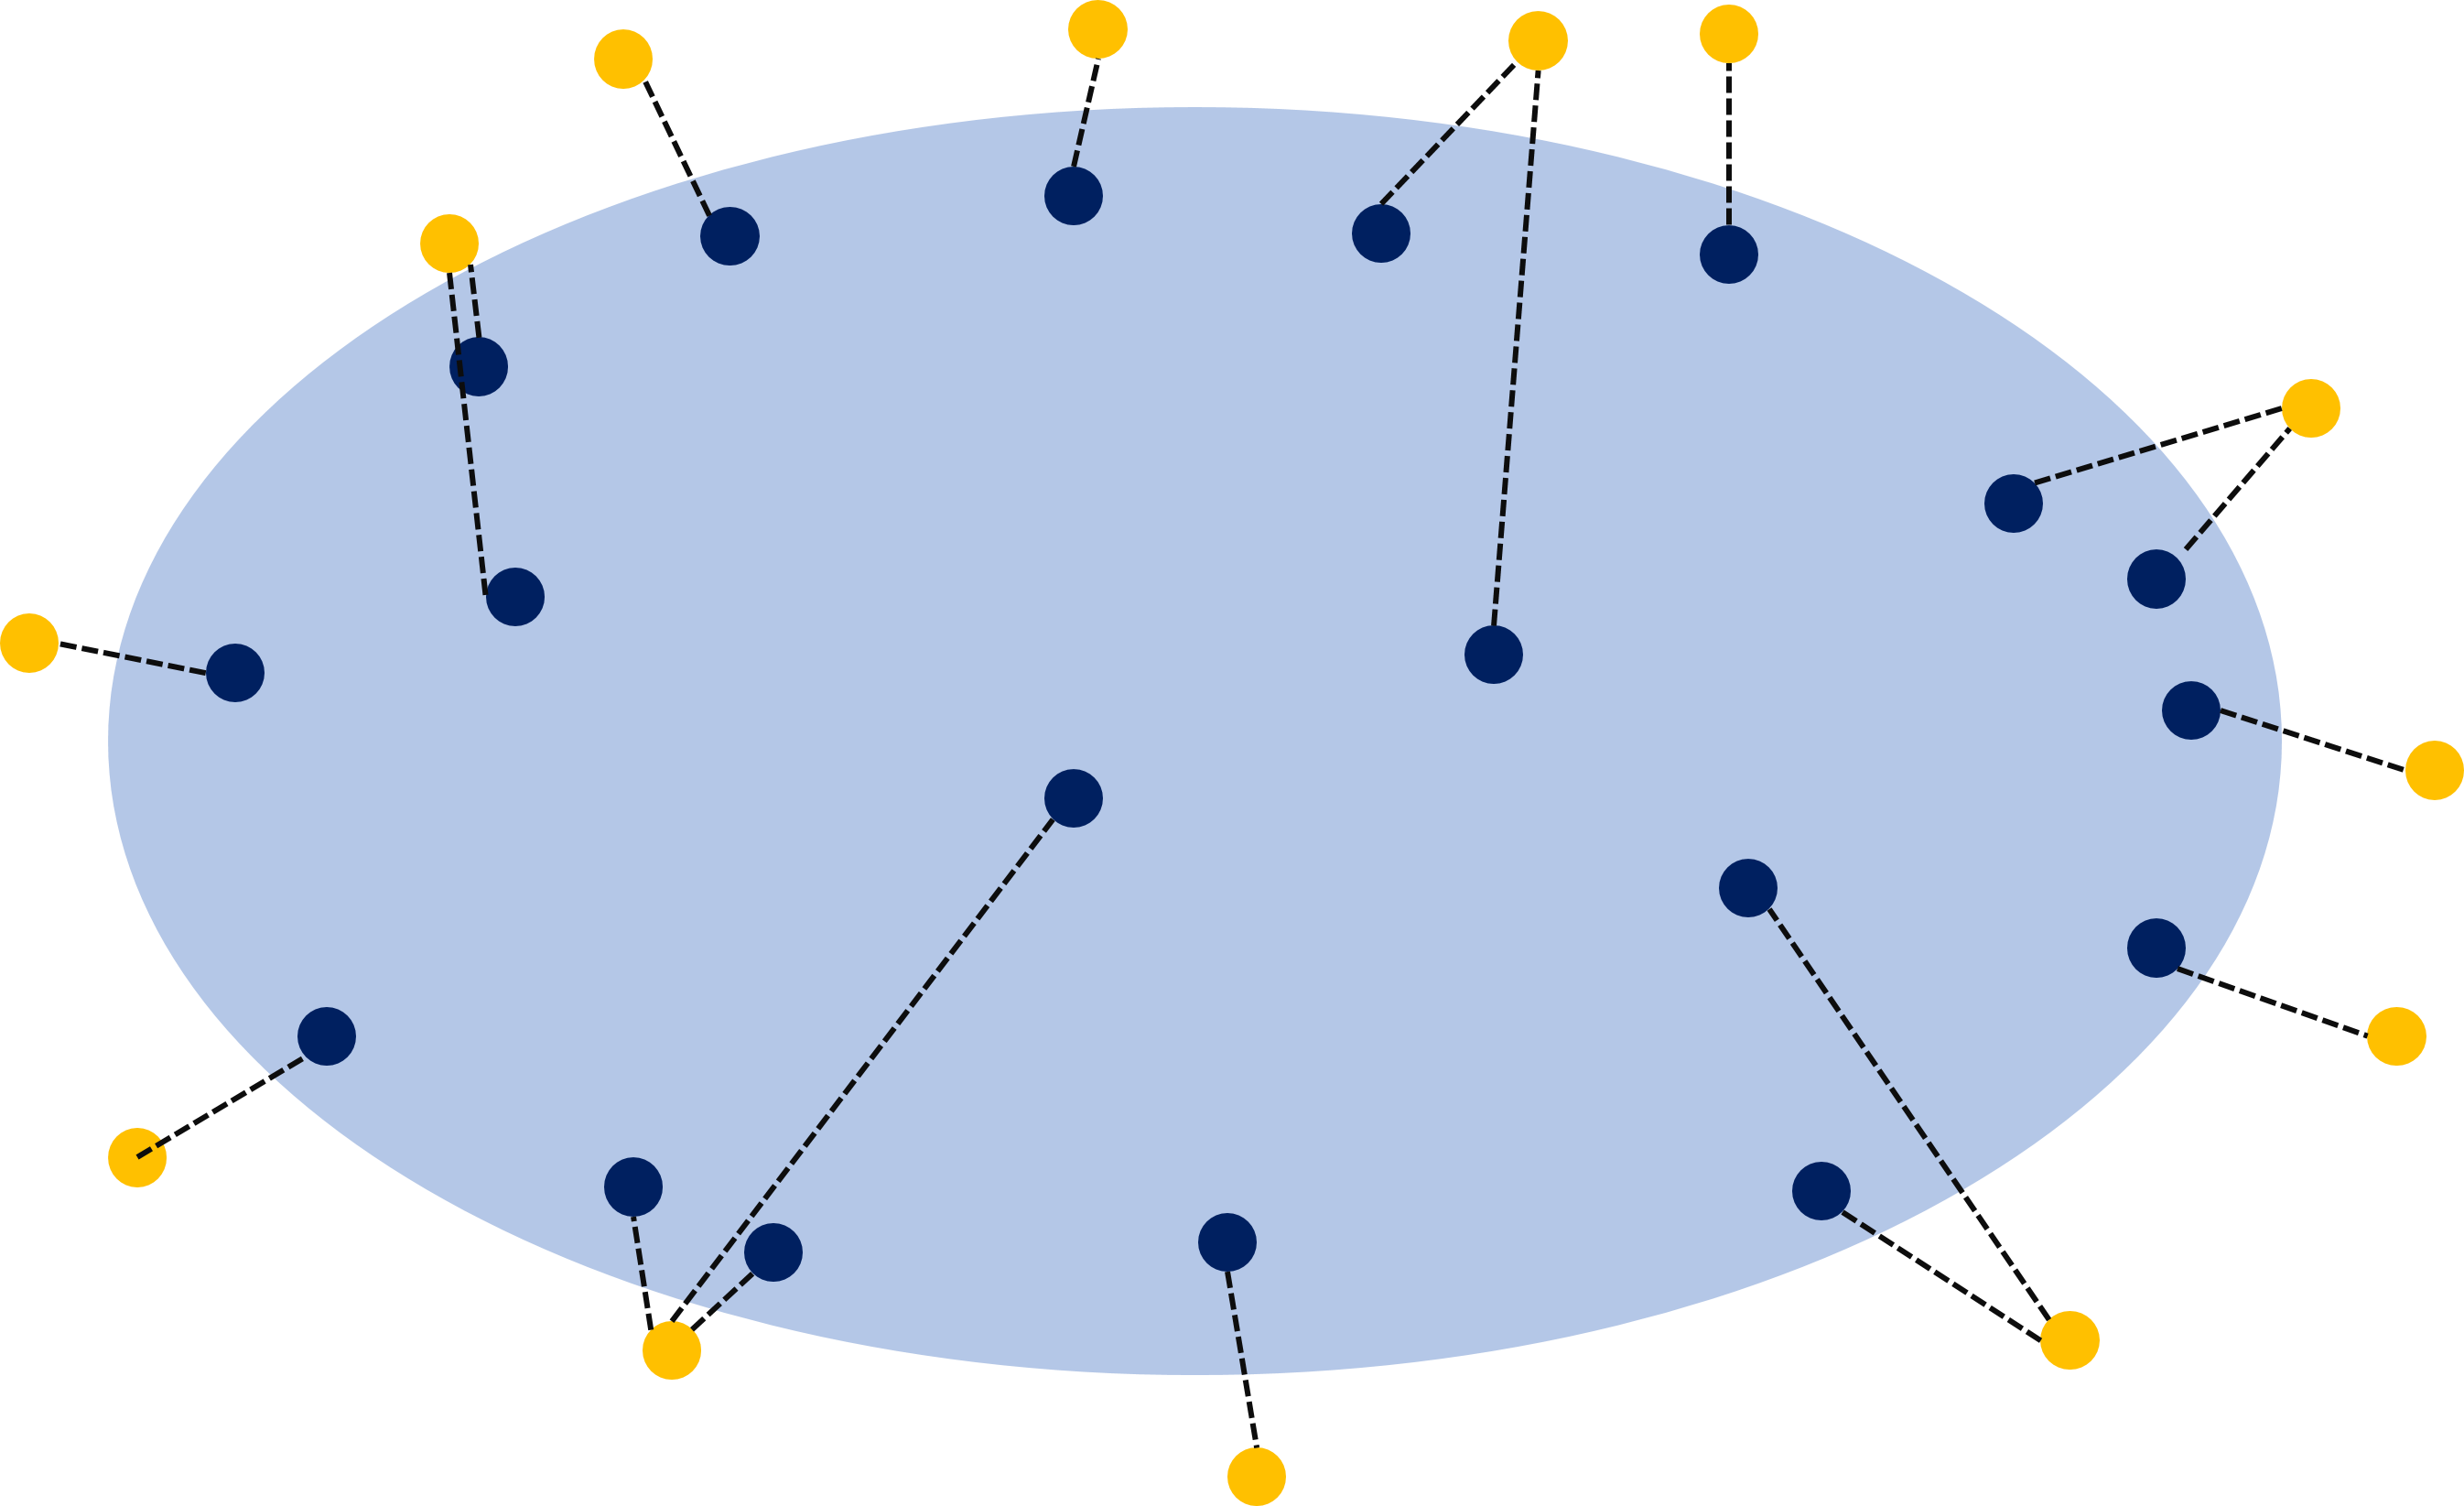
\includegraphics[width=\textwidth]{S4-Explicabilite_globale/figures/filtre4.png}
      \caption{Seuls les vecteurs supports appariés sont conservés.} \label{fig:filtre4}
    \end{subfigure}

\caption{Illustration des principes des différentes étapes de filtre. L'ellipse bleue correspond aux éléments d'une classe observée. Les points bleus appartiennent à la classe considérée, ce sont des éléments protagonistes. Les points jaunes appartiennent aux autres classes, ils sont antagonistes. Les points gris sont ceux supprimés à chaque étape. } \label{fig:filtre}
\end{figure}

Les deux dernières étapes sont illustrées dans la figure~\ref{fig:filtre}. La suppression des doublons consiste à ne conserver qu'un seul point au cas où plusieurs seraient au même endroit, et n'est donc pas visible sur cette illustration.
Dans le contexte One \textit{vs.} Rest, les points de la classe étudiée sont situés à l'intérieur de l'ellipse bleue. Les points en dehors de cette ellipse peuvent être de toutes les autres classes.
Les sous figures~\ref{fig:filtre1} et~\ref{fig:filtre2} montrent le filtre sur les vecteurs supports. Les points grisés en figure~\ref{fig:filtre1}  sont les points candidats qui ne sont pas des vecteurs supports.
% TODO Harold : je ne mettrai pas de gris, mais tous les points soit bleu soit gris. avec une frontière différente (pointillée) pour montrer les frontières du MO. ensuite en b on a le svm avec ses frontières et ses SV.
La figure~\ref{fig:filtre2} présente le même espace avec ces points de données en gris supprimés.
La figure~\ref{fig:filtre3} montre l'appairage entre chaque vecteur support protagoniste et le vecteur support antagoniste le plus proche. Un vecteur support antagoniste peut ainsi être apparié à plusieurs vecteurs supports protagonistes. Cette étape permet de conserver \textit{au maximum} $2*P$ vecteurs supports, avec $P$ le nombre de vecteurs supports protagonistes.
Pour appliquer ce filtre, il faut dans un premier temps entraîner un SVM.
% Approche SVM

\paragraph{Entraînement du SVM}
Avec le SVM entraîné, nous nous concentrons sur les vecteurs supports. Les vecteurs supports sont des points de données intéressants utilisés par le SVM pour apprendre sa fonction de décision.

%  Tout d'abord, comprenons mieux les informations que nous voulons extraire.
%
% \begin{figure}[h!tpb]
%  \centering 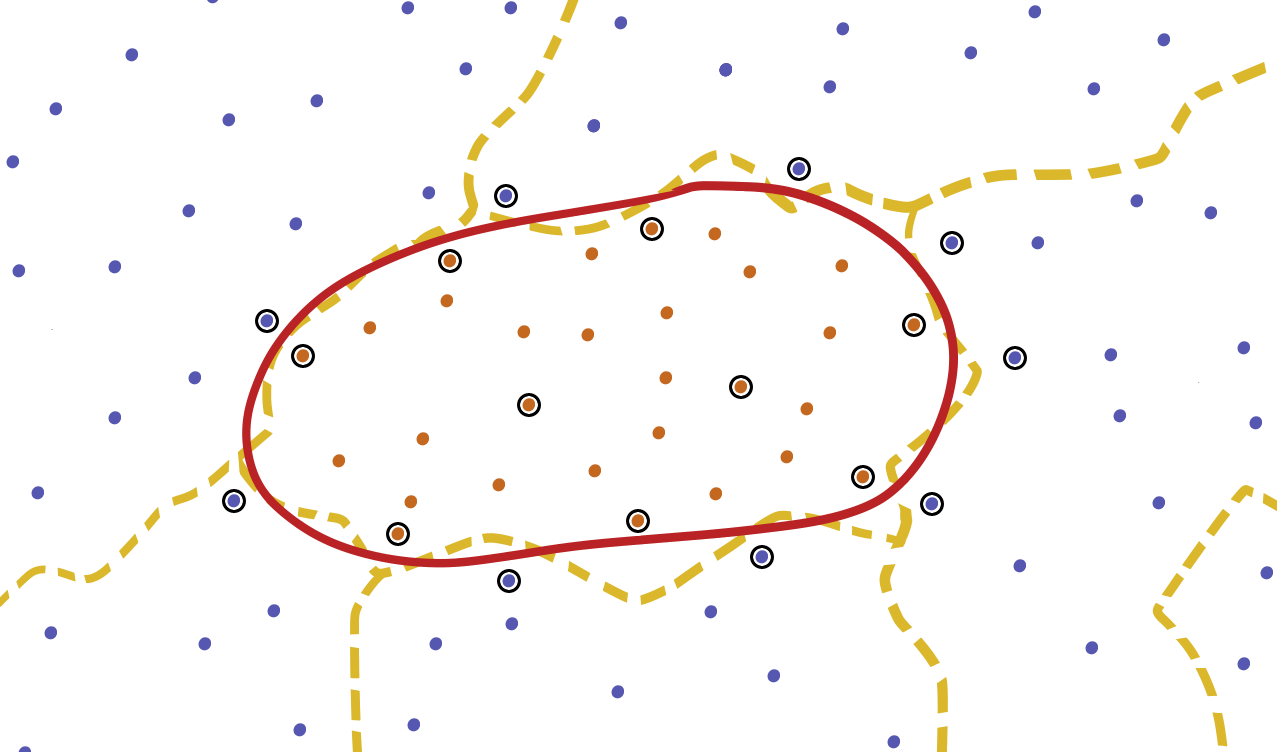
\includegraphics[width=0.8\textwidth]{S4-Explicabilite_globale/figures/svm_frontiere.png}
% \caption{Classification entre une classe A (points orange) et les autres (points bleus). La frontière de décision exacte du modèle original, en pointillés jaunes, n'est pas tangible. La frontière rouge représente l'hyperplan du SVM pour la classe A. Les vecteurs supports délimitant cet hyperplan sont entourés en noir. } \label{fig:svm_decision_boundaries}
% \end{figure}
%
% La Fig.~\ref{fig:svm_decision_boundaries} montre comment obtenir une meilleure idée d'une frontière de décision approximative, en visualisant les vecteurs supports du SVM. Toutes les lignes pointillées jaunes illustrent la représentation mentale de l'utilisateur des limites de décision du MO.
%
% Les points orange et bleus représentent respectivement les instances d'une classe étudiée A et les instances de toutes les autres classes. Tous les points encerclés en noir sont les vecteurs supports du SVM. Ils aident à déterminer la limite de décision du SVM pour cette classe A, représentée dans la Fig.\ref{fig:svm_decision_boundaries} par une ligne rouge.

% Cette frontière est rendue compréhensible pour les humains en observant des exemples intéressants caractérisant la décision du MO.
% Le coût de la précision pour obtenir cette explicabilité est supporté par le SVM et non par la MO.

La figure~\ref{fig:model_architecture} compare les architectures du MO, sur la première ligne et du SVM sur la seconde. Pour un MO donné, l'architecture des premières couches est conservée, et devient la vectorisation en seconde ligne. La classification est effectuée par un SVM à noyau gaussien. Pour que le SVM copie le MO, il doit être entraîné sur les décisions de classification du MO. L'entrée du MO correspond aux données réelles $(X,Y)$, $X$ étant les données vectorisées et $Y$ étant la classe. Il produit en sortie une décision $\bar{Y}$. L'entraînement du SVM prend la même entrée $X$, mais la cible est $(\bar{Y})$ : il est entraîné dans les résultats de classification du MO. Le jeu de données d'entraînement est le même ou à défaut un sous-ensemble.

\begin{figure}[h!tpb]
\centering 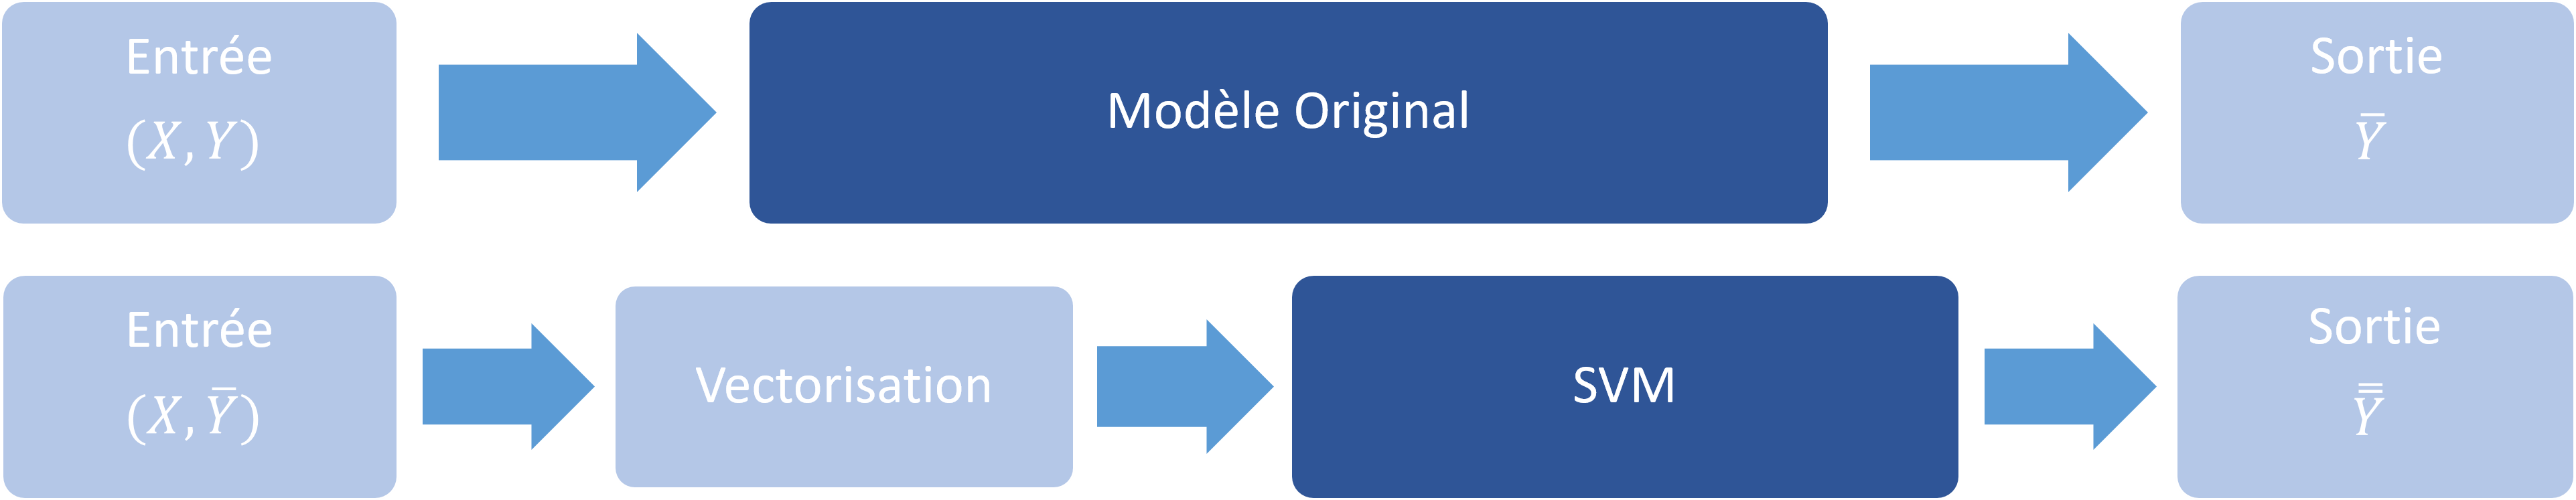
\includegraphics[width=\textwidth]{S4-Explicabilite_globale/figures/model_architecture.png}
\caption{Comparaison entre le modèle boîte noire et les architectures SVM. L'entrée du SVM est basée sur la sortie du modèle original.} \label{fig:model_architecture}
\end{figure}

Les vecteurs supports du SVM ainsi déterminés sont appariés par classe, un vecteur positif avec son vecteur négatif le plus proche. Cette liaison donne des couples pertinents d'exemples factuels et contre-exemples pour une classe donnée.

\paragraph{Les vecteurs support}
Le SVM est composé de $n-1$ classifieurs One \textit{vs.} Rest. Chacun de ces classifieurs est une fonction de décision, basée sur des vecteurs supports $SV$. Son signe de sortie correspond à une classe (positif) ou au reste (négatif). La fonction de décision pour une instance $x$ est :

\begin{equation}
\sum_{i \in SV}y_i\alpha_i K(x_i,x)+b
\end{equation}

Avec $K$ la fonction noyau gaussienne :

\begin{equation}
   K(x_i, x) = e^{-\gamma||x_i-x||}
\end{equation}

Les coefficients duaux des vecteurs supports $y_i\alpha_i $ sont définis avec leur signe $y \in \{-1,1\}$ et leur valeur $\alpha \geq 0$. Ils peuvent être positifs (protagonistes) : pour une classe, le label du vecteur support est le même. Ils peuvent aussi être négatifs : leur étiquette diffère de la classe donnée.

Un classifieur peut, selon le cas d'utilisation, avoir de nombreux vecteurs supports, en particulier avec des coefficients $y$ négatifs. En associant à chaque vecteur positif le vecteur négatif le plus proche, nous éliminons les vecteurs négatifs non associés. Dans le cadre de l'analyse de textes, nous utilisons la distance cosinus.

Pour fournir une vision claire à l'utilisateur, il est nécessaire de trier les points les plus pertinents parmi les vecteurs supports, qui sont déjà les points les plus pertinents du jeu de données d'apprentissage.

\subsection{Tri} \label{C4:tri}

Le tri proposé permet de fournir un résumé digeste pour un humain. L'objectif est donc de ressortir un ensemble de moins d'une dizaine de couples d'exemples. Il est possible de laisser la main à l'utilisateur ou utilisatrice, afin de lui laisser choisir le niveau de zoom qu'iel souhaite.

% SVM
Encore une fois, de nombreuses techniques sont à notre disposition. Il est possible de se baser sur le SVM et trier les couples de vecteurs par somme de leurs valeurs alpha. Il est également possible de prendre un point de la classe étudiée (exemple) au hasard, et effectuer une approximation polygonale en passant par une heuristique gloutonne de sélection du point le plus éloigné du point précédent, ou du barycentre des points sélectionnés.

% CAH
Nous proposons de regrouper les exemples négatifs, en un nombre réduit de groupes. Nous discuterons dans la suite d’une méthode permettant de calculer de tels groupes. Pour chaque groupe constitué, un seul élément est conservé. Ce mécanisme permet d'assurer une bonne répartition des exemples et contre-exemples sélectionnés.

\begin{figure}[h!tpb]
    % \begin{subfigure}{1\textwidth}
    %   \centering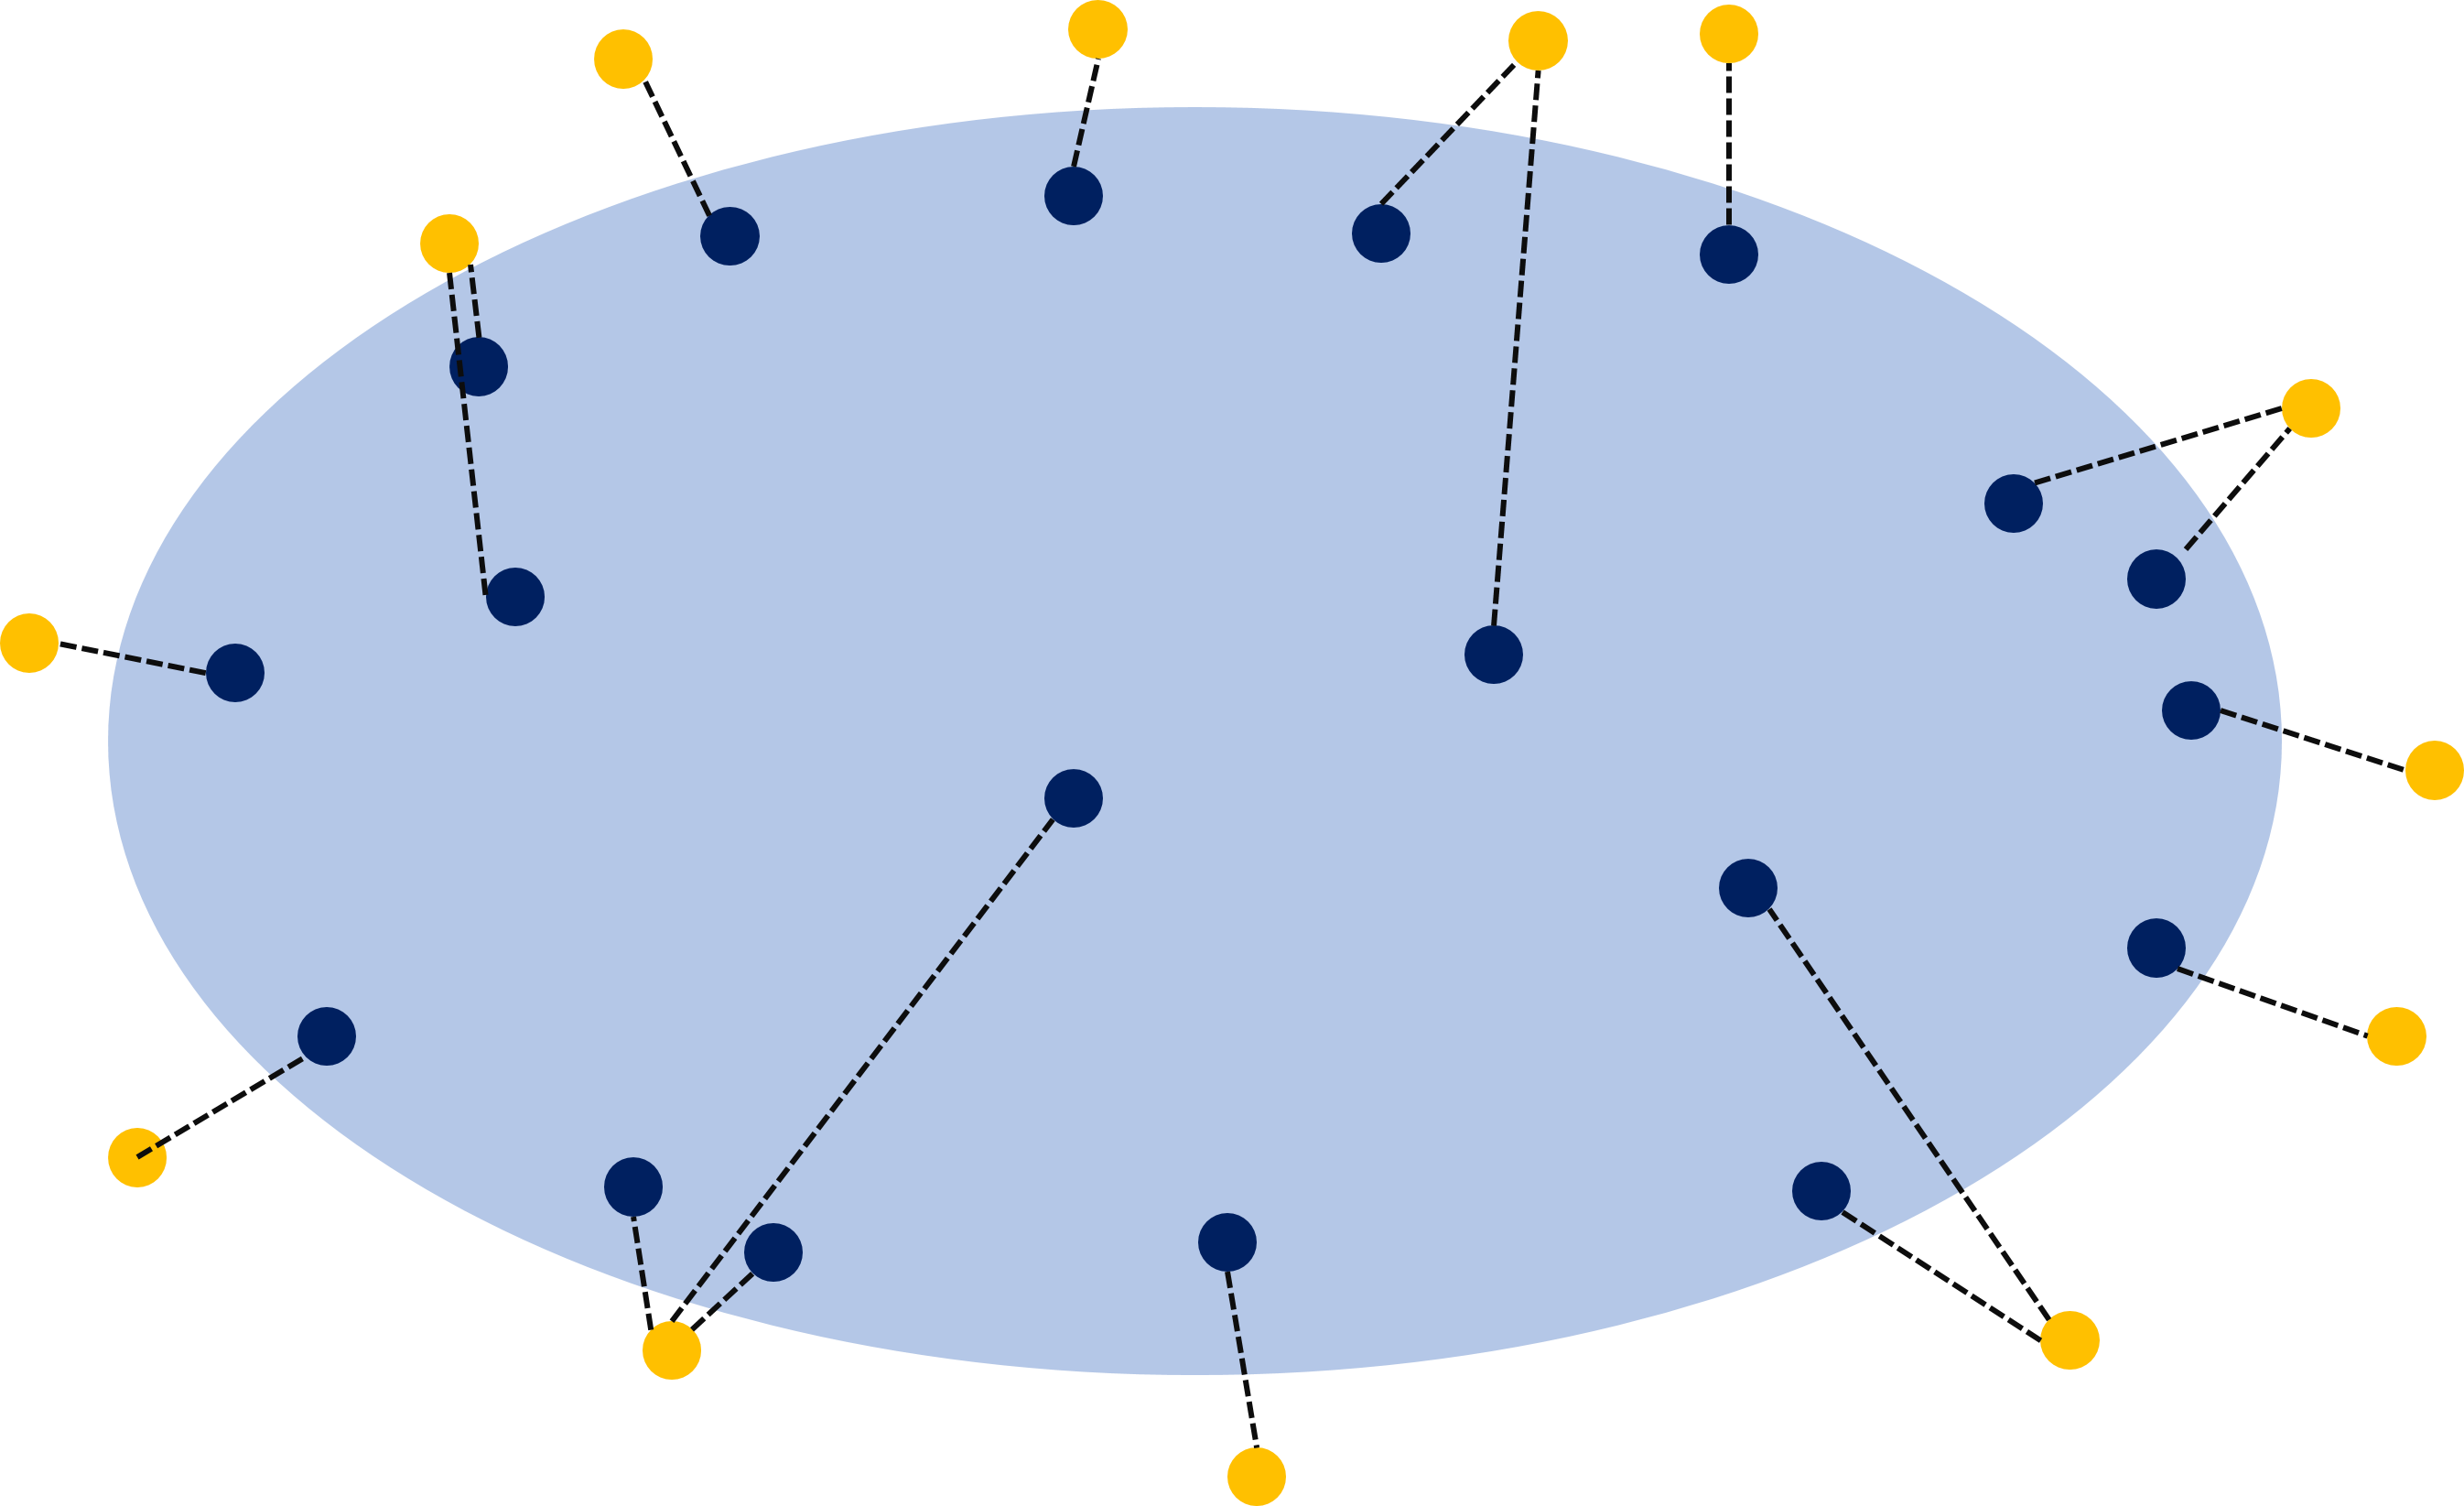
\includegraphics[width=0.5\textwidth]{S4-Explicabilite_globale/figures/filtre4.png}
    %   \caption{[Optionnel] Ensemble des vecteurs supports protagonistes et antagonistes de la classe analysée, représentés avec leurs appairages.} \label{fig:tri0}
    % \end{subfigure}
    \begin{subfigure}[t]{0.45\textwidth}
      \centering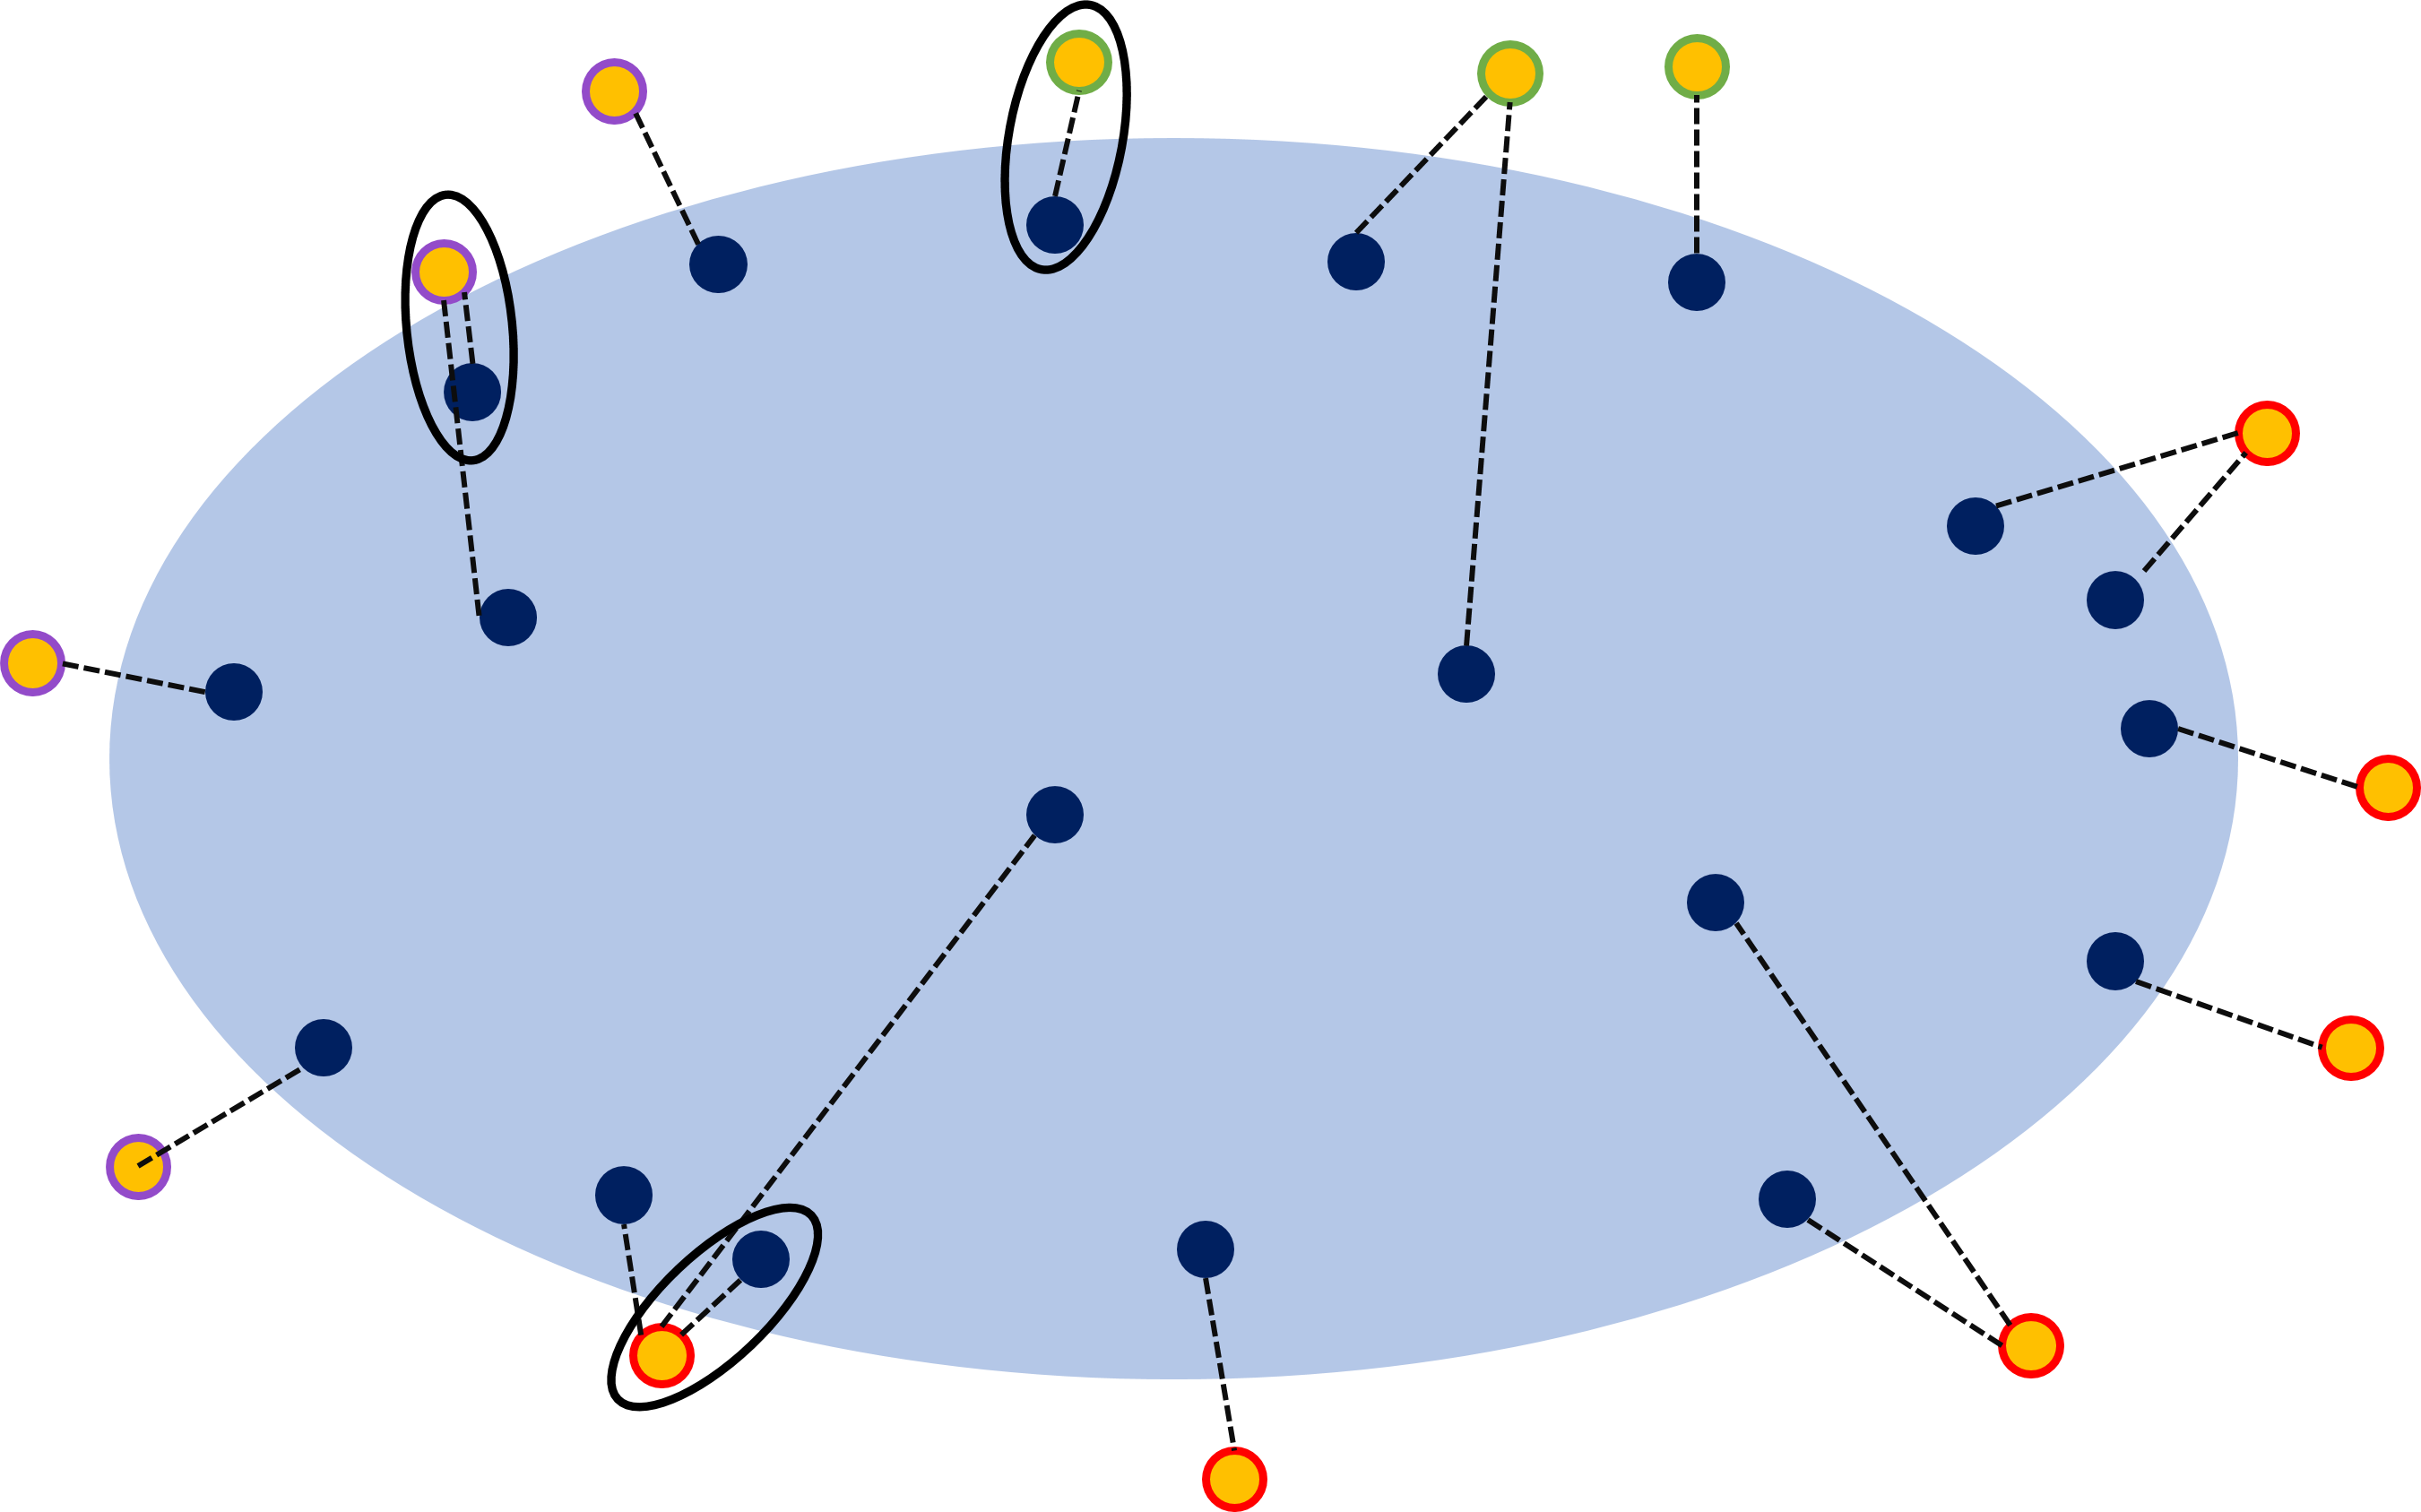
\includegraphics[width=\textwidth]{S4-Explicabilite_globale/figures/tri1.png}
      \caption{Regroupement des vecteurs supports antagonistes en 3 groupes par une méthode quelconque: violet, vert et rouge. Pour chaque groupe, la paire de distance minimale est entourée.} \label{fig:tri1}
    \end{subfigure} \qquad
    \begin{subfigure}[t]{0.45\textwidth}
      \centering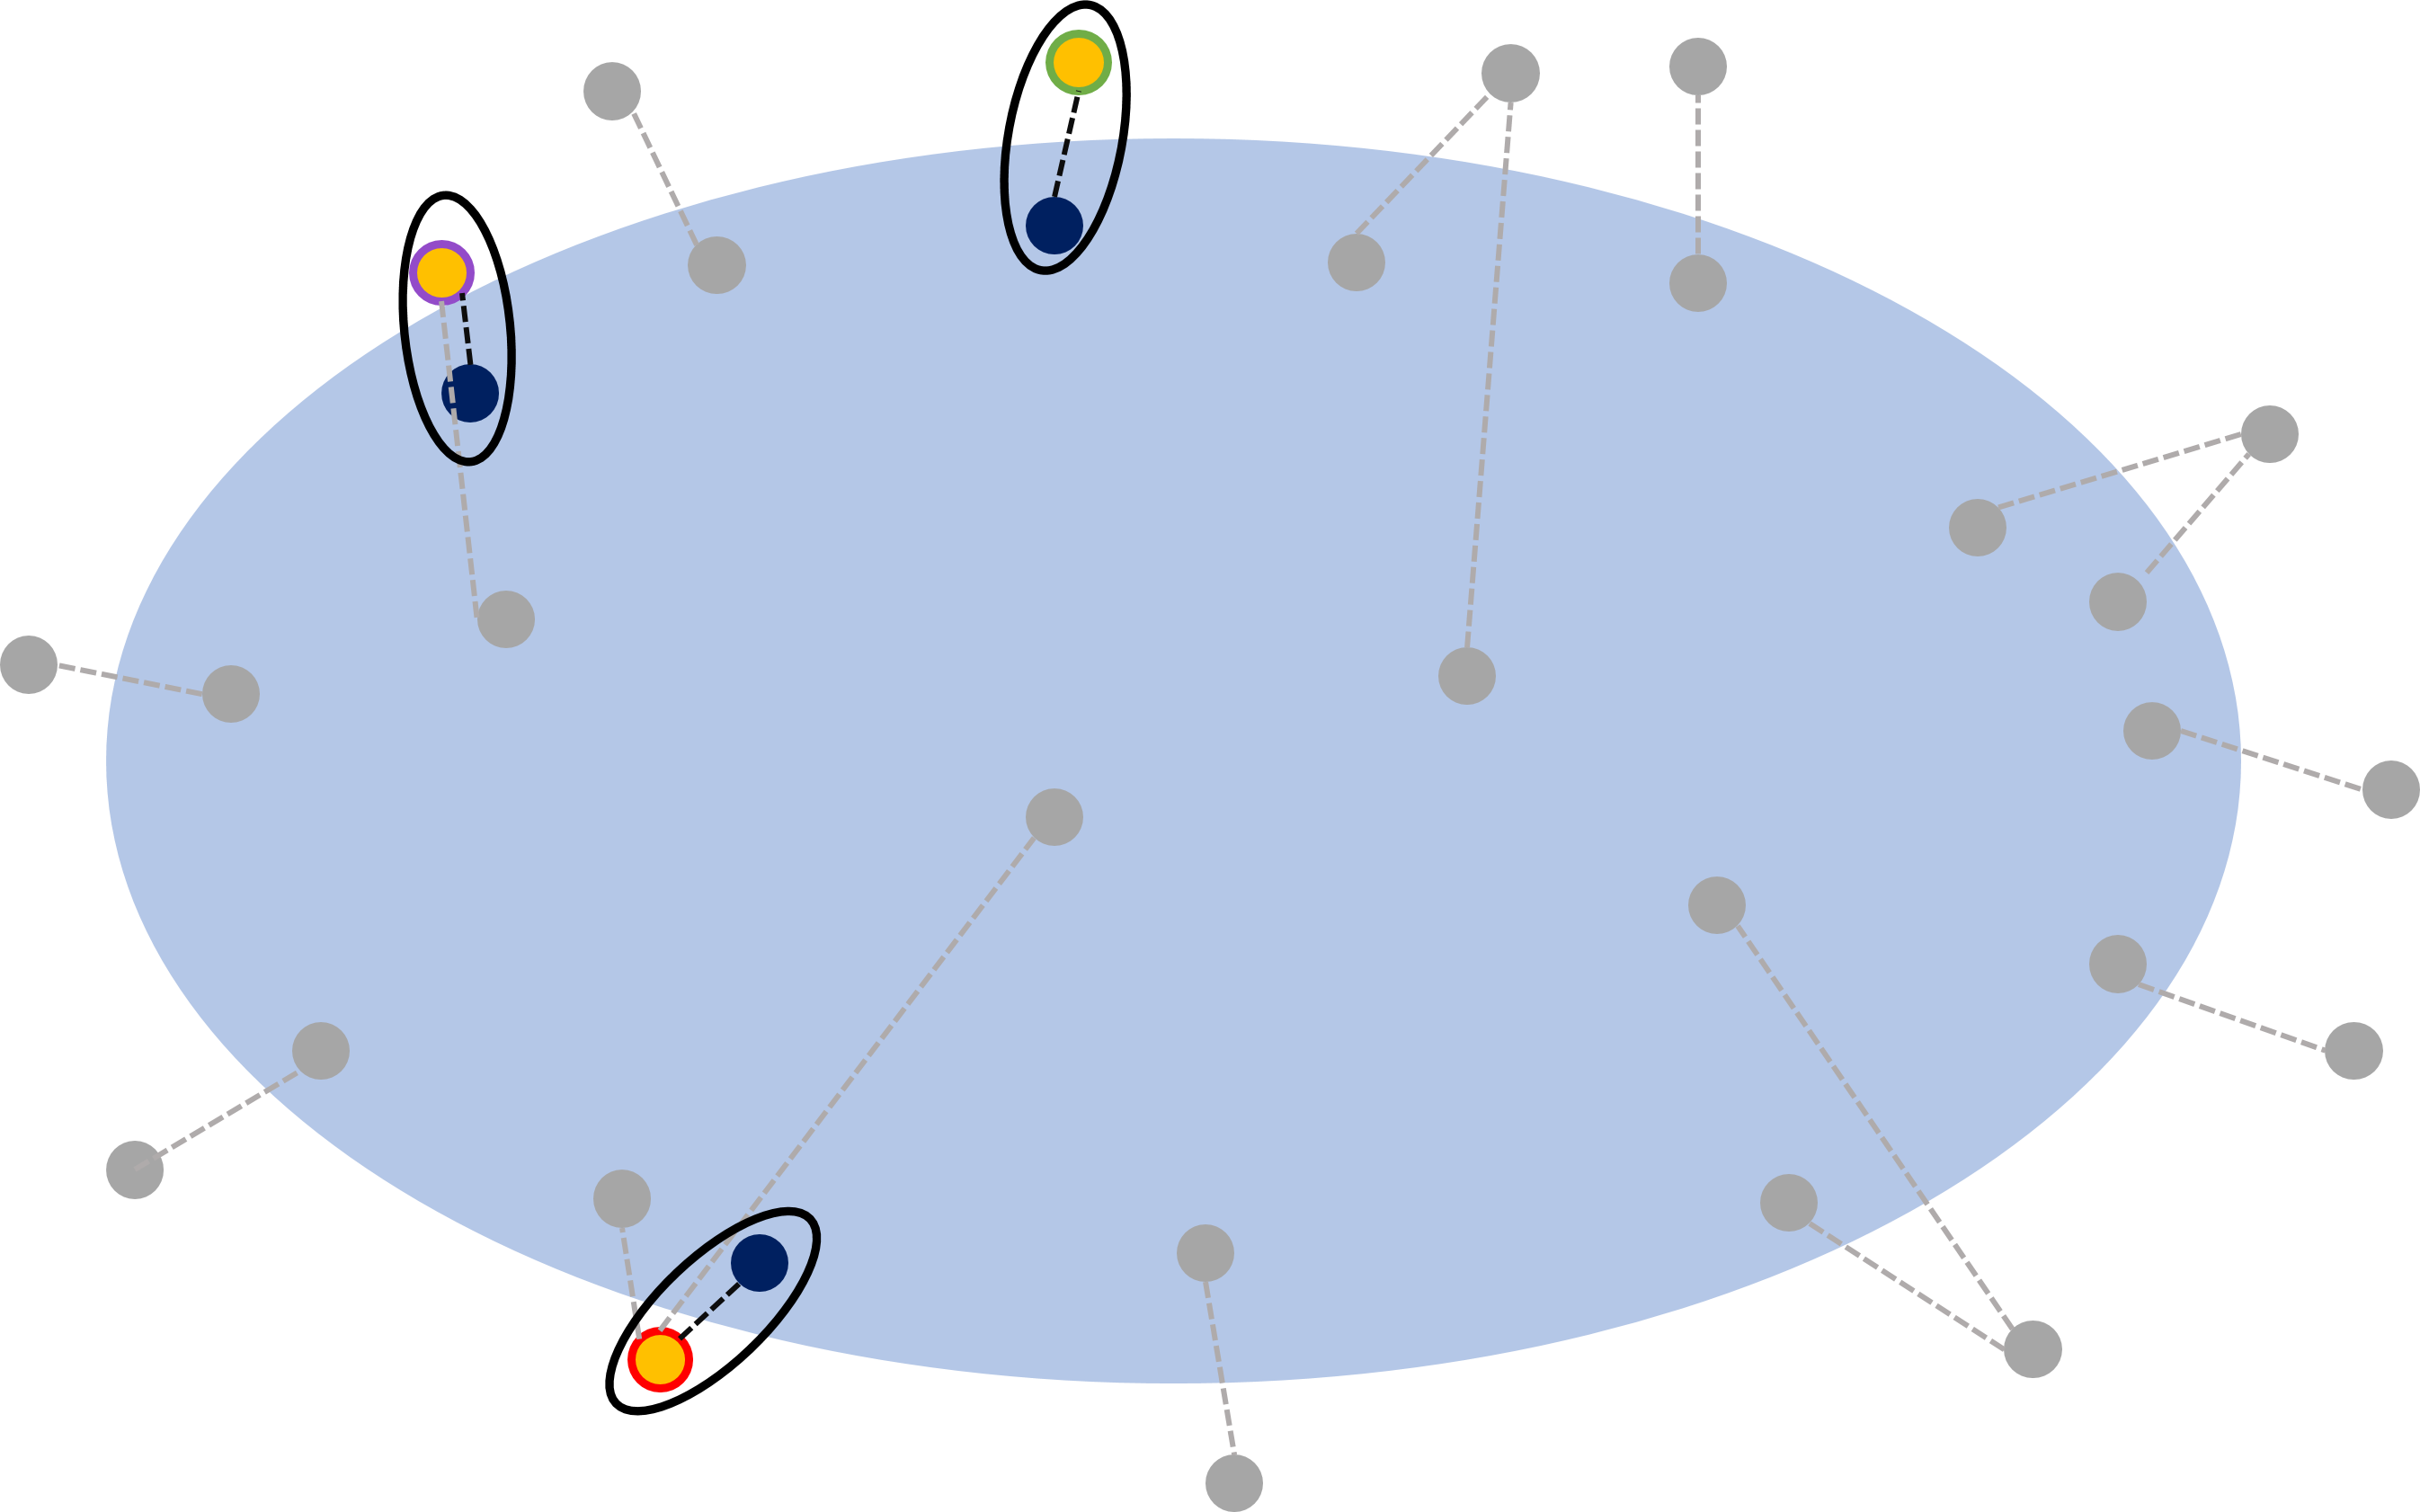
\includegraphics[width=\textwidth]{S4-Explicabilite_globale/figures/tri2.png}
      \caption{Seules les paires entourées sont conservées, les autres points sont mis de côté.} \label{fig:tri2}
    \end{subfigure}

    \begin{subfigure}[t]{0.45\textwidth}
      \centering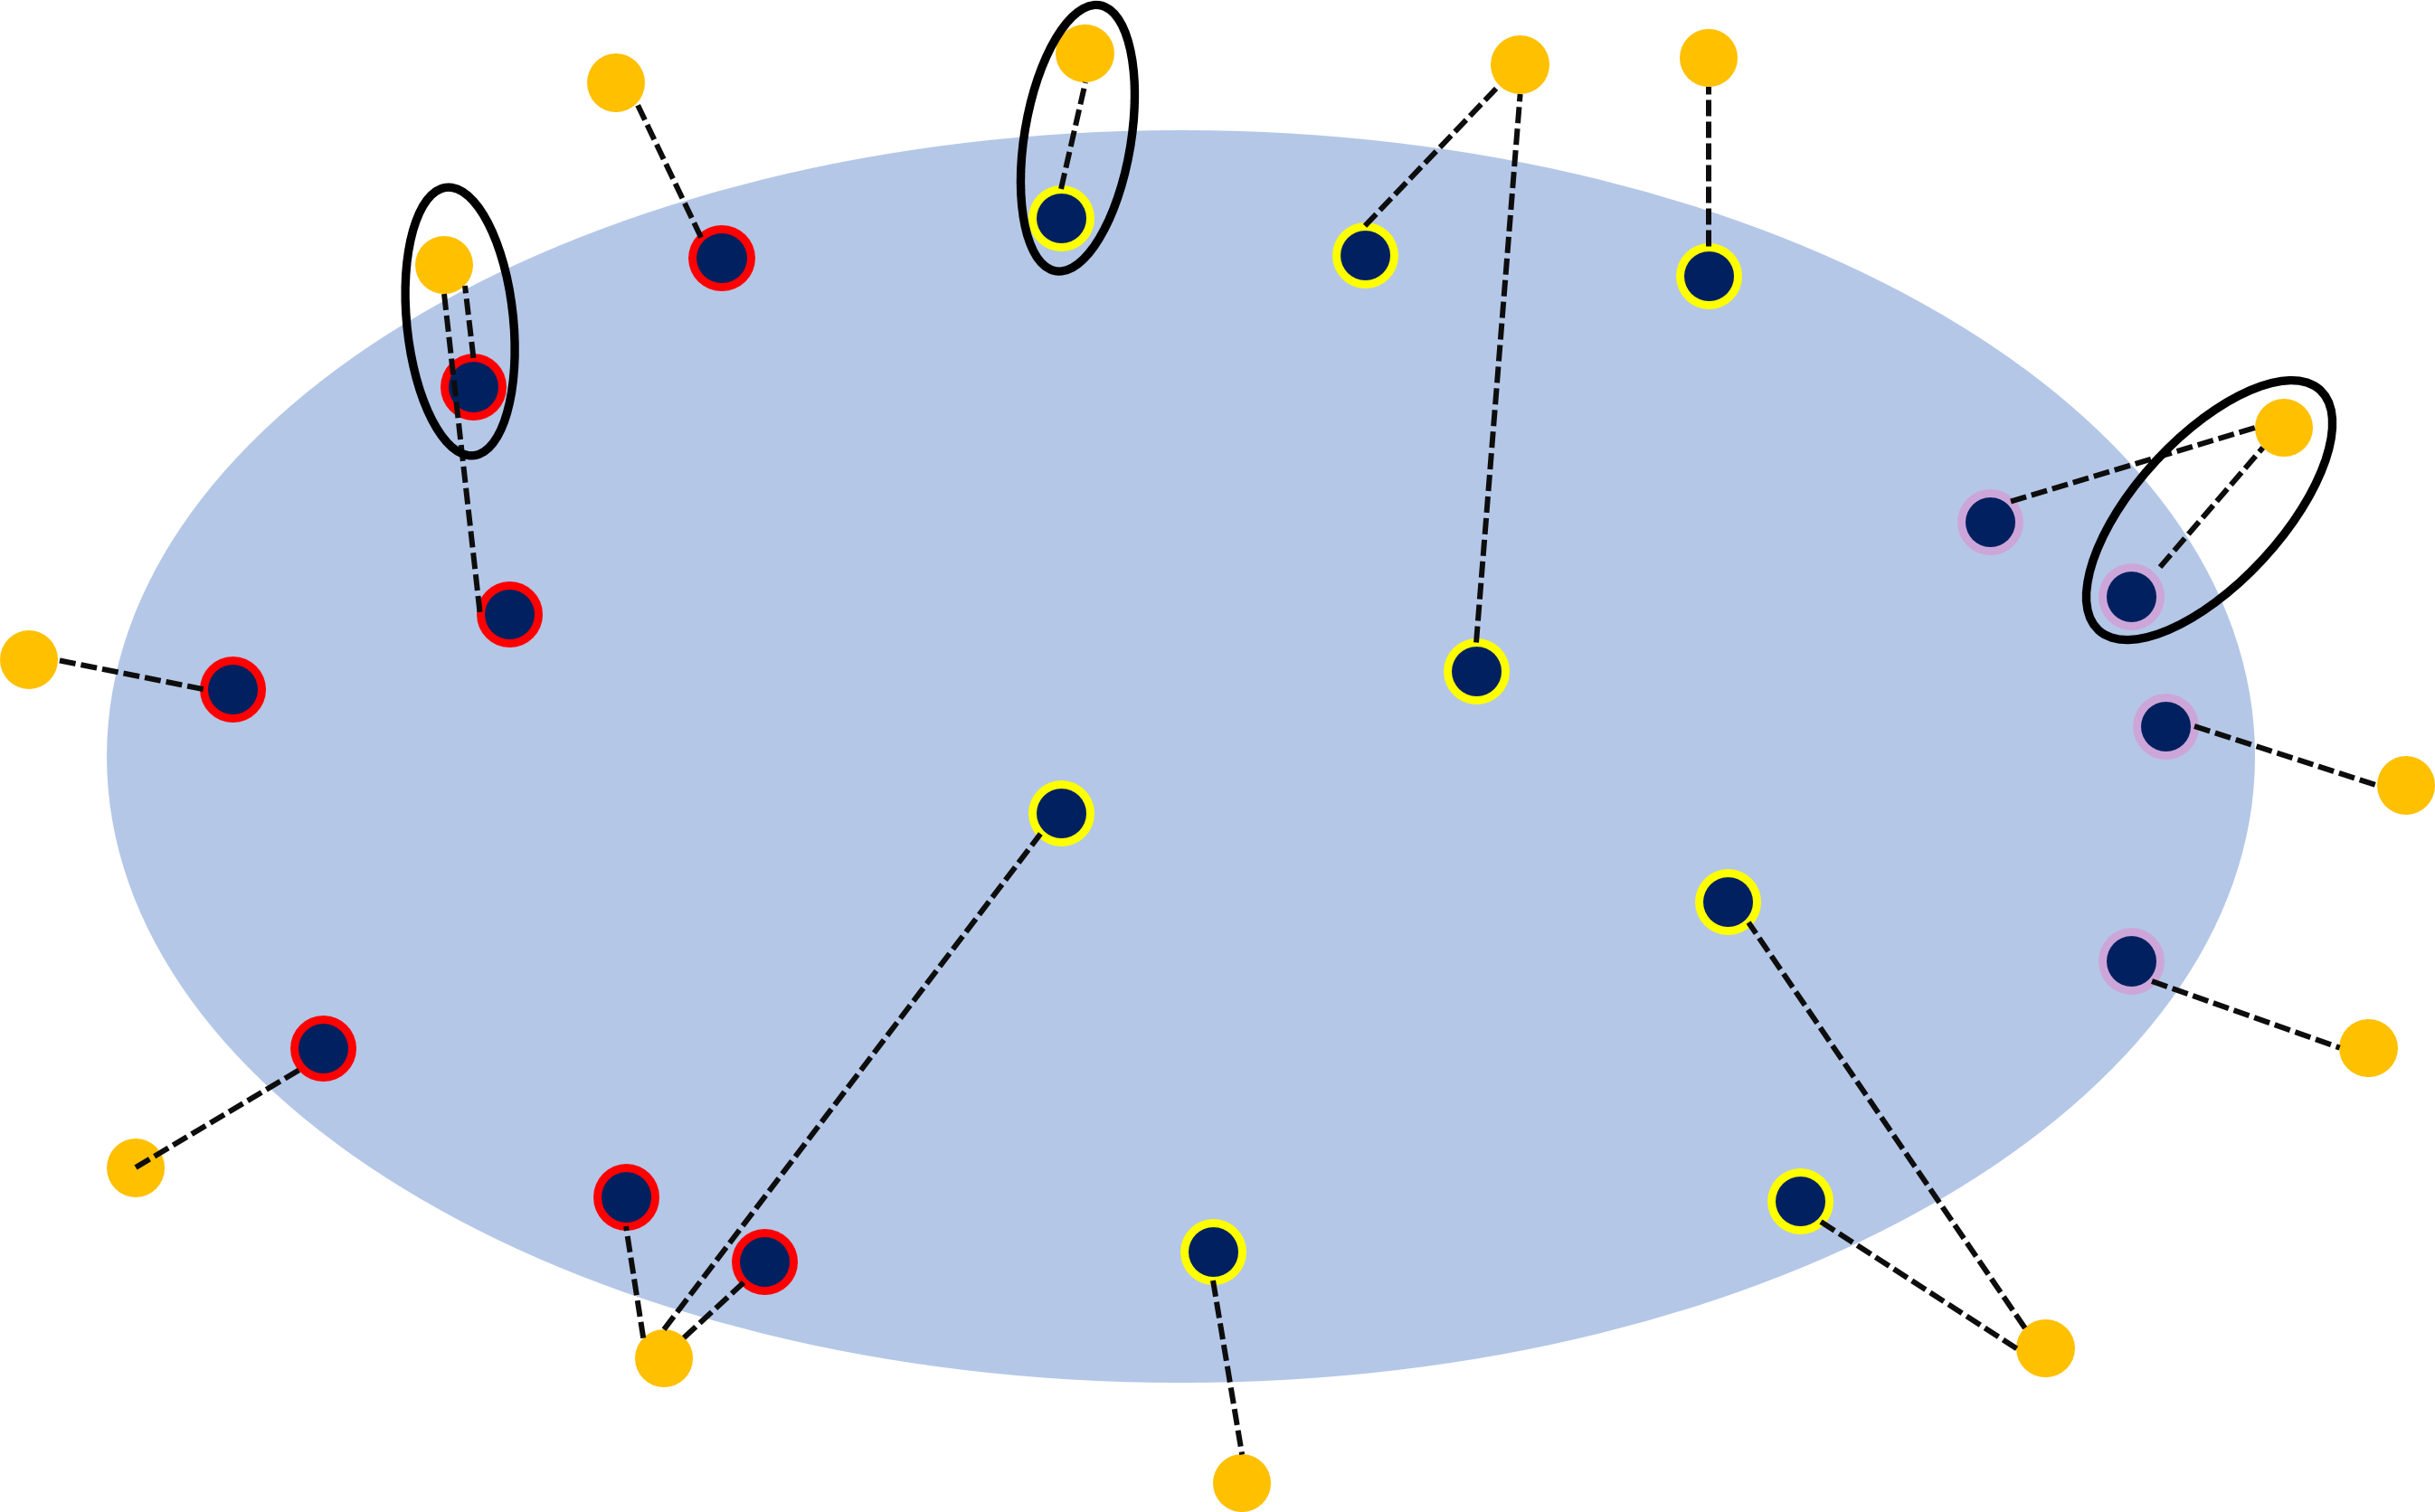
\includegraphics[width=\textwidth]{S4-Explicabilite_globale/figures/tri3.png}
      \caption{Regroupement des vecteurs supports protagonistes en 3 groupes par une méthode quelconque: violet, jaune et rouge. Pour chaque groupe, la paire de distance minimale est entourée.}
      \label{fig:tri3}
    \end{subfigure} \qquad
    \begin{subfigure}[t]{0.45\textwidth}
      \centering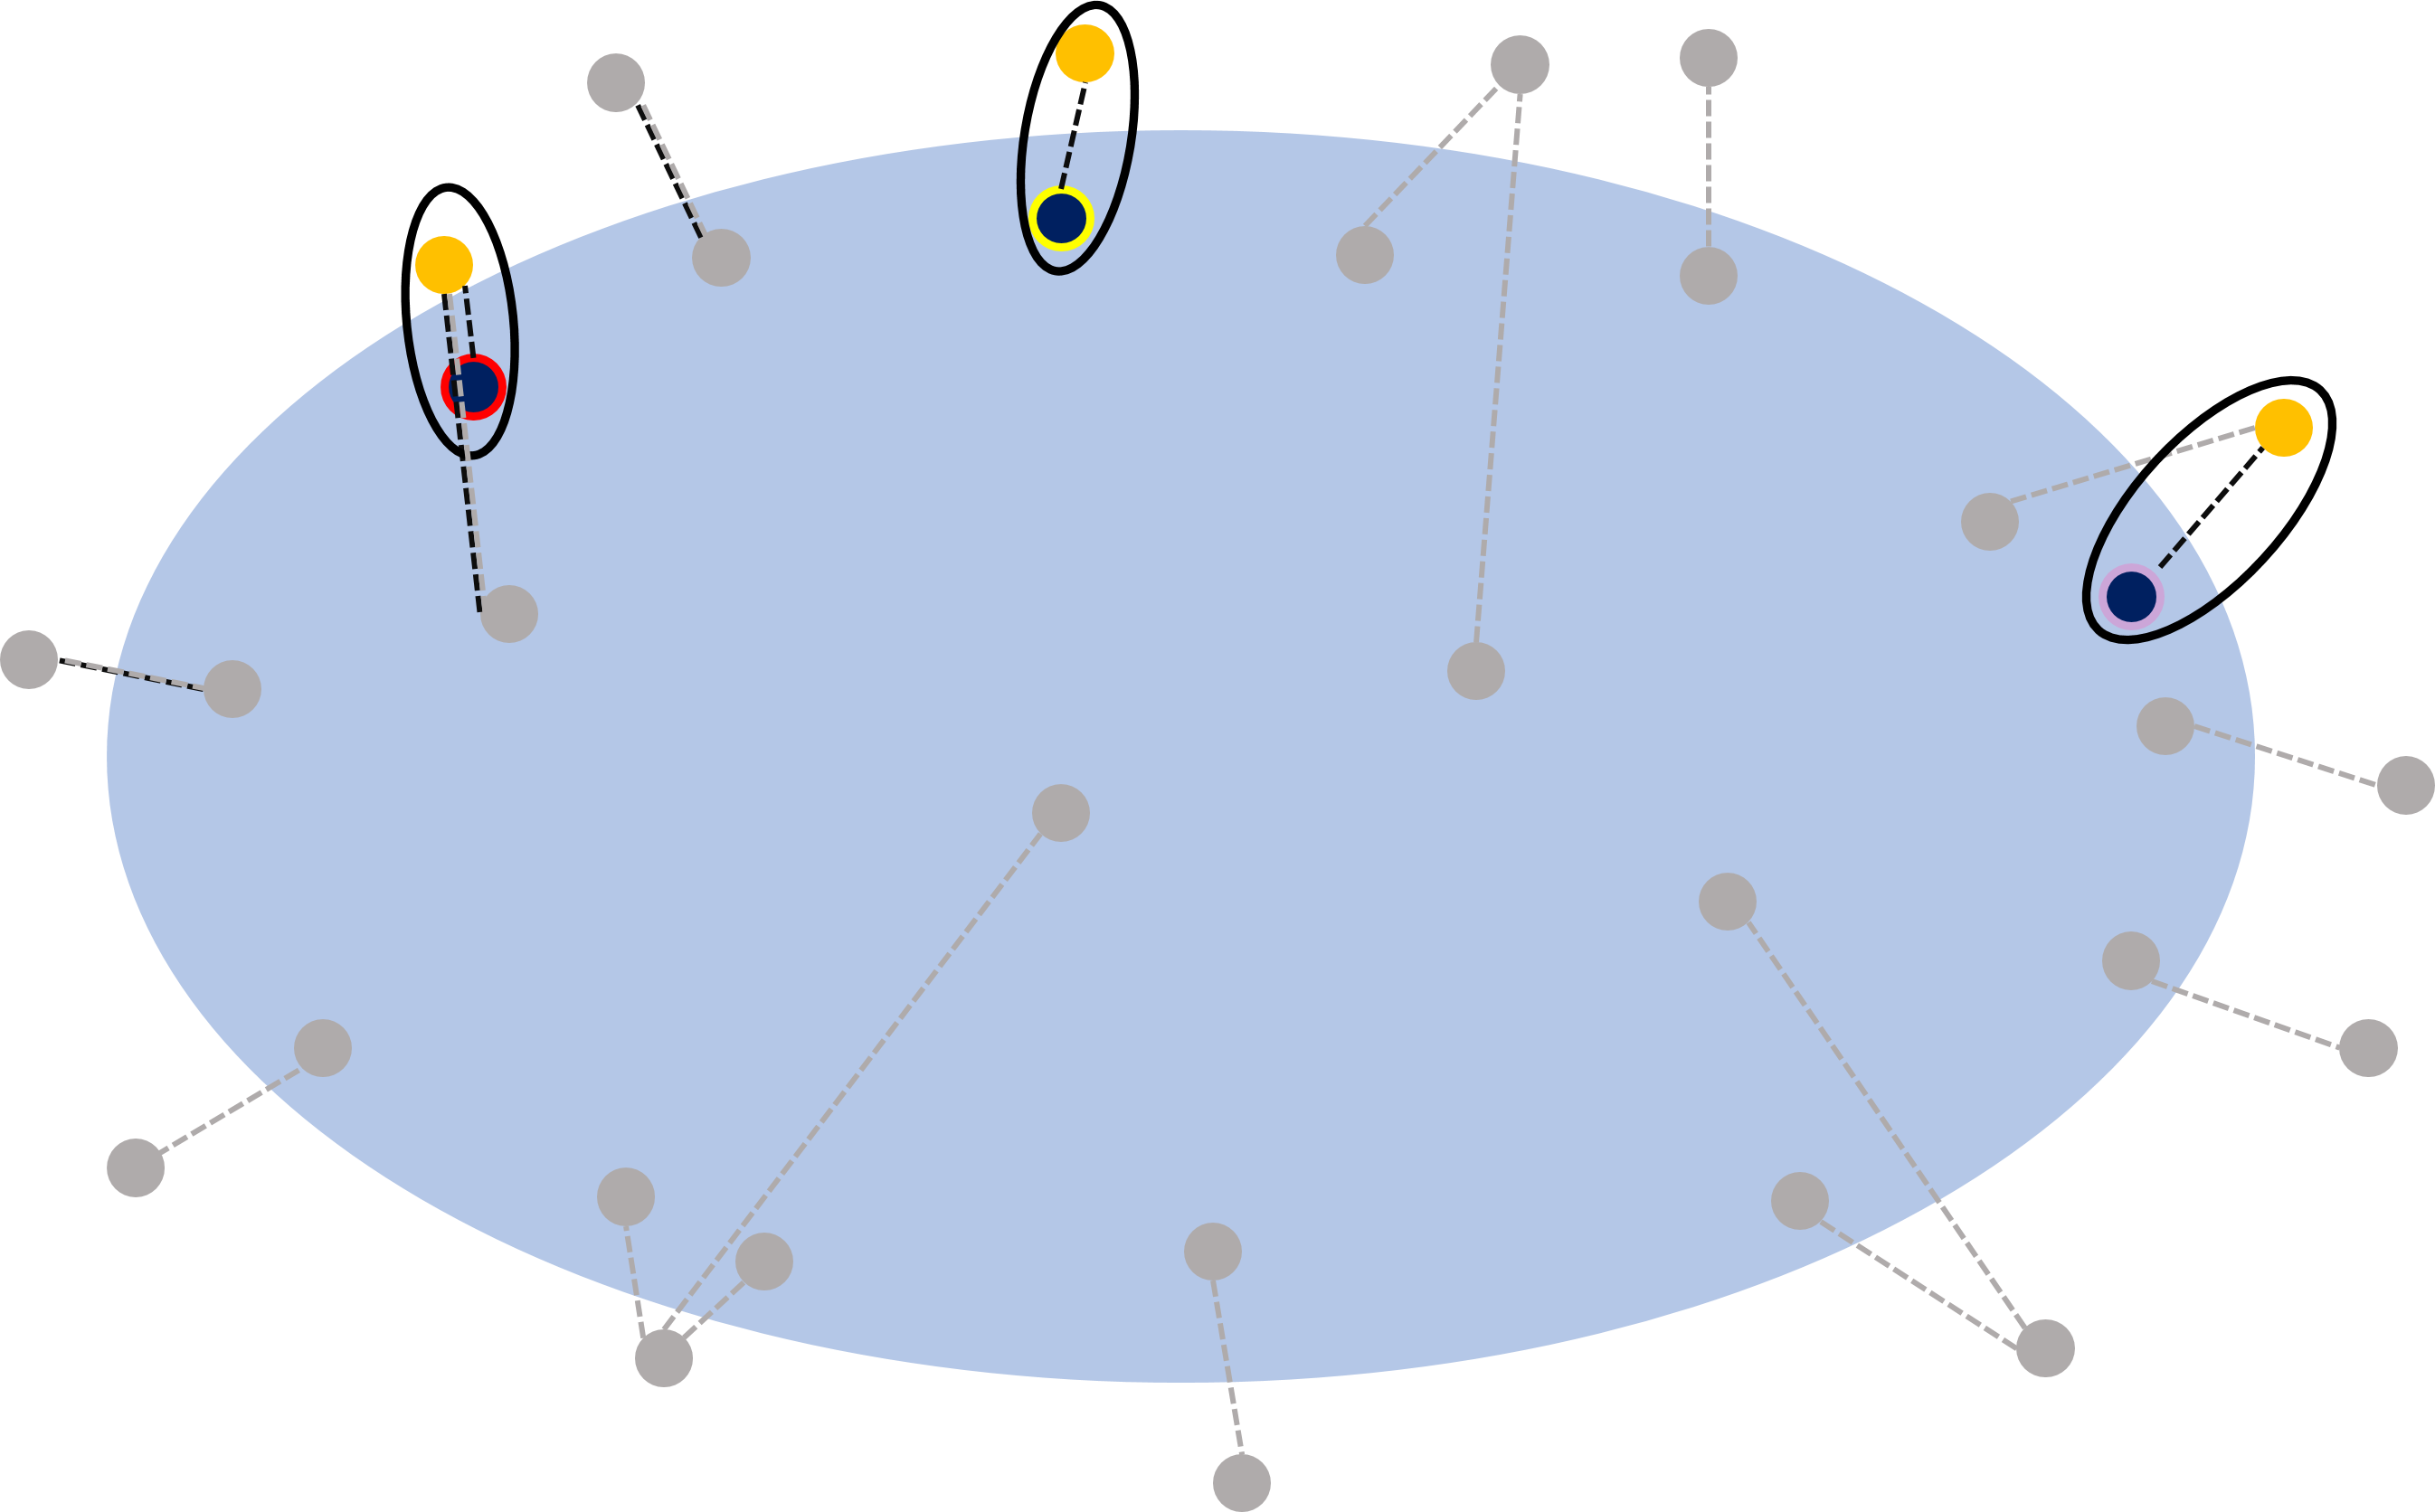
\includegraphics[width=\textwidth]{S4-Explicabilite_globale/figures/tri4.png}
      \caption{Seules les paires entourées sont conservées, les autres points sont mis de côté.} \label{fig:tri4}
    \end{subfigure}

    \caption{Illustration des différentes étapes de tri. } \label{fig:tri}
\end{figure}

La figure~\ref{fig:tri} présente le filtre avec la sélection de $n=3$ paires d'exemples et contre-exemples. Les figures~\ref{fig:tri1} et~\ref{fig:tri2} présentent le premier mode du filtre en effectuant les regroupements sur les vecteurs supports antagonistes. Les figures~\ref{fig:tri3} et~\ref{fig:tri4} présentent le second mode du filtre en effectuant les regroupements sur les vecteurs supports protagonistes.
Pour chaque mode, le principe est identique. Les vecteurs supports (protagonistes ou antagonistes) sont regroupés en $n$ groupes. Pour chaque groupe, le couple d'éléments de distance minimale est présenté, c'est à dire les instances les plus proches de la frontière. Tous les autres éléments sont mis de côté.

Il est également possible de concaténer les résultats des deux modes. La sélection des paires de distance intra paire minimale augmente la probabilité que les paires sélectionnées soient identiques entre les deux modes de regroupements. Si $n$ paires sont demandées, le nombre de paires concaténées des deux modes sera alors compris entre $n$ et $2n$.

Le regroupement est effectué par une Classification Ascendante Hiérarchique (CAH) basée sur le critère de Ward.
Une heuristique classique afin de déterminer le nombre de groupes à conserver consiste à observer le dendrogramme présentant les regroupements et la distance interclasses. La meilleure découpe de ce dendrogramme est classiquement celle apportant le plus d'informations, c'est à dire celle où le saut est le plus important. Nous considérons la CAH comme un zoom, et laissons l'utilisateur couper où iel le souhaite. Les couples d'exemples ainsi sélectionnés sont présentés.

Cette méthode permet de présenter un ensemble restreint et représentatif des couples d'exemples et contre-exemples d'intérêt. Il revient alors à l'utilisateur d'effectuer l'analyse des éléments pour la classe étudiée. Ce travail est à faire pour toutes les classes afin d'obtenir une vision globale du modèle.

% Transition
Maintenant que le protocole est défini, il est appliqué à un cas d'utilisation réel, ce qui nous permet de voir ses avantages, ses limites et ses possibilités d'amélioration.

\section{Application} \label{C4:application}

Nous appliquons cette stratégie de caractérisation au cas d'usage LEGO présenté en chapitre~\ref{C3}. Pour rappel, c'est un problème de classification multi-classes, mono-label, par phrase. Il y a 26 classes, l'une d'entre elles comprenant les phrases légales. Cette classe a un intérêt fonctionnel tout particulier : elle correspond à des phrases ``correctes'', là où tous les autres motifs sont des phrases ``incorrectes''.

Le modèle étudié pour cette application est le modèle à attention présenté en chapitre 3. Dans ce chapitre, le modèle à attention est considéré comme une boîte noire. Les données candidates de la section~\ref{C4:candidats} sont les données d'entraînement présentées en chapitre 3. L'implémentation du filtre présentée précédemment est appliquée en section~\ref{C4:app_filtre}. Celle du tri est appliquée en section~\ref{C4:app_tri}.

\subsection{Filtre} \label{C4:app_filtre}

% Caractéristiques de MO
Le SVM entraîné est un SVC de sci-kit learn, avec un noyau gaussien. L'ensemble d'apprentissage est le même que celui utilisé pour le MO, mais la classe à prédire est la décision du MO, comme spécifié dans~\ref{C4:filtre}. Il obtient une précision moyenne de $0,997$, signifiant qu'il parvient à imiter le MO.

Le SVM possède 14840 vecteurs support, correspondant à $3,09\%$ de l'ensemble de données d'apprentissage. Les vecteurs supports correspondent à 12077 vecteurs uniques, soit $2,52\%$ de l'ensemble de données d'apprentissage. Certaines phrases de l'ensemble d'apprentissage sont des doublons, d'où la légère variation. Dans notre analyse, nous avons élagué les doublons en sélectionnant le premier de tous les vecteurs supports correspondant à une phrase donnée.

Pour chaque classe, des vecteurs supports sont sélectionnés, divisés en vecteurs supports positifs et négatifs. Une distance cosinus est calculée entre les deux groupes. Comme nous cherchons à retrouver la proximité sémantique des phrases, nous utilisons la distance cosinus. Un vecteur support positif (resp. négatif) donne un exemple factuel (resp. contrefactuel) pertinent. Chaque exemple factuel pertinent de la classe étudiée est apparié avec l'exemple contrefactuel le plus proche.

\begin{table}
    \caption{Exemples factuels pertinents et leurs exemples contrefactuels pour la classe ``Discrimination : contrat étudiant''. La décision du MO associée au contrefactuel et la distance entre l'exemple factuel et le contrefactuel sont également affichées.} \label{tab:results_student}
    \begin{tabular}{|p{0.32\textwidth}|p{0.5\textwidth}|p{0.13\textwidth}|}
        \hline
        \textbf{Exemple factuel } & \textbf{Exemple contrefactuel associé (CFE)} & \textbf{Distance cosinus} \\ \hline
        Profil recherché : Etudiant(e), salarié(e), retraité(e). & Etudiant(e), retraité(e), travaillant à temps partiel ou en recherche d'emploi, vous êtes avant tout passionné(e) par les enfants ? Devenez un(e) nounou Kangourou ! & $0,066$ \\ \hline
        Etudiants acceptés. & 35 H/Semaine minimum Etudiants acceptés. & $0,050$ \\ \hline
    \end{tabular}
\end{table}

La table~\ref{tab:results_student} présente deux couples d'exemples factuels et contrefactuels pour la classe \textit{``Discrimination : contrat étudiant''}. Il est illégal en France de spécifier que le candidat d'une offre d'emploi doit être un étudiant.

\begin{table}
    \caption{Diminution des paires pour la classe \textit{``Discrimination : Contrat étudiant''}}  \label{tab:combinatoire}
    \begin{tabular}{|p{0.3\textwidth}|p{0.15\textwidth}|p{0.28\textwidth}|p{0.22\textwidth}|}
        \hline
         & \textbf{Légal} & \textbf{Contrat étudiant} & \textbf{Paires} \\ \hline
        Données brutes             & 385754  & 2477 & 955 512 658 \\ \hline
        \multicolumn{4}{|l|}{Suppression des doublons}              \\ \cline{1-4}
        Vecteurs uniques           & 259 853 & 841  & 218 536 373 \\ \hline % facteur 4,4
        \multicolumn{4}{|l|}{Sélection des vecteurs supports}        \\ \hline
        vecteurs supports           & 4 688   & 151  & 707 888     \\ \hline % facteur 309
        \multicolumn{4}{|l|}{Appairage par similarité cosinus}       \\ \hline
        Paires de vecteurs supports & 43      & 151  & 151         \\ \hline % facteur 4 688
    \end{tabular}
\end{table}

Pour cette classe, nous obtenons $151$ couples de vecteurs supports positifs et négatifs. Le tableau~\ref{tab:combinatoire} montre les réductions consécutives du nombre de points  en partant du nombre de données brutes). La dernière colonne présente le nombre de paires possibles. Avant le filtre, le nombre de paires d'exemples et contre-exemples dans les données d'entraînement pour la classe \textit{Discrimination : Contrat étudiant} est proche du milliard. Pour cette classe spécifiquement, la suppression des doublons divise le nombre de paires par $4$ environ. La sélection des vecteurs supports divise par $309$ ce nombre, et l'appairage final le divise par $4 688$.
Cette réduction est notable sur toutes les classes étudiées, et est plus prononcées sur les classes fortement représentées, comme le montre le tableau~\ref{tab:nb_vs}.

\begin{table}
    \caption{Nombre de vecteurs supports protagonistes uniques et de paires d'exemples et contre-exemples obtenus grâce au filtre, par classe. } \label{tab:nb_vs}
    \begin{tabular}{|p{0.65\textwidth}|p{0.15\textwidth}|p{0.1\textwidth}|}
        \hline
            \textbf{Classe}    & \textbf{VS uniques} & \textbf{Paires} \\ \hline
            Discrimination : Activité syndicale ou mutualiste      &     8  &  8      \\ \hline
            Discrimination : Age                                   &  2251  &  579    \\ \hline
            Discrimination : Apparence physique                    &   590  &  311    \\ \hline
            Discrimination : Contrat aidé                          &    15  &  14     \\ \hline
            Discrimination : Contrat étudiant                      &   841  &  151    \\ \hline
            Discrimination : \'Etat de santé                       &  5815  &  1006   \\ \hline
            Discrimination : Grossesse                             &    43  &  30     \\ \hline
            Discrimination : Handicap                              &   674  &  296    \\ \hline
            Discrimination : M\oe urs                              &   102  &  62     \\ \hline
            Discrimination : Nationalité                           &   168  &  123    \\ \hline
            Discrimination : Opinions politiques                   &    27  &  22     \\ \hline
            Discrimination : Origine                               &   349  &  193    \\ \hline
            Discrimination : Résidence                             &  1845  &  369    \\ \hline
            Discrimination : Genre - Au moins un accord au féminin &  1247  &  415    \\ \hline
            Discrimination : Genre - Intitulé exclusivement féminin &  2606  &  478   \\ \hline
            Discrimination : Genre - Mention genre exclusif        &   129  &  84     \\ \hline
            Discrimination : Situsation familiale                  &    29  &  26     \\ \hline
            Discrimination : Taille                                &   173  &  101    \\ \hline
            Droit du travail : Achat de matériel                   &  6018  &  892    \\ \hline
            Droit du travail : CDD Possibilité CDI                 & 12461  &  1154   \\ \hline
            Libertés : Casier Judiciaire                           &   351  &  117    \\ \hline
            Libertés : Tenue vestimentaire                         &    22  &  18     \\ \hline
            Légal                                                  & 259853 &  4688   \\ \hline
            Offre non conforme : Stage                             &   115  &  78     \\ \hline
            Terme innaproprié                                      &  2974  &  650    \\ \hline
            Texte spécifique : Gratuité                            &   377  &  212    \\ \hline
    \end{tabular}
\end{table}

Le tableau~\ref{tab:nb_vs} présente le nombre de vecteurs supports protagonistes uniques, ainsi que le nombre de paires finales pour chaque classe du cas d'usage. Pour l'ensemble des classes correspondant à des motifs de rejet, l'étape de filtre permet d'obtenir entre $8$ et $1 154$ paires d'exemples et contre-exemples. La classe de phrases légales en comporte $4 688$, ce qui est justifié par sa nature plus générale.

Afin de présenter un nombre digeste d'exemples et contre-exemples, il faut effectuer un tri supplémentaire, présenté dans la section suivante.

\subsection{Tri} \label{C4:app_tri}

% Choix nb groupes
La CAH permet d'obtenir une représentation hiérarchique sous la forme d'un dendrogramme. La figure~\ref{fig:dendrogramme} présente le dendrogramme obtenu grâce à la  CAH des 151 vecteurs supports protagonistes de la classe ``\textit{Discrimination : contrat étudiant}''. Le dendrogramme est affiché pour $n=10$ groupes, puisqu'il n'est pas souhaitable de montrer plus d'éléments aux utilisateurs et utilisatrices.

\begin{figure}[h!tpb]
 \centering 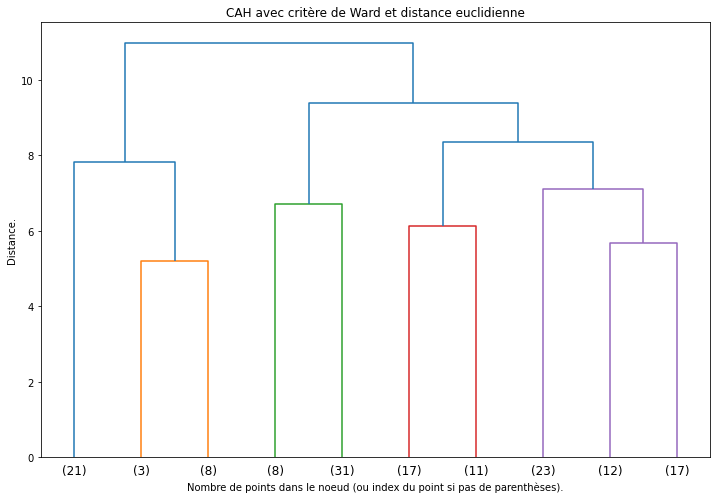
\includegraphics[width=\textwidth]{S4-Explicabilite_globale/figures/dendrogramme.png}
\caption{Dendrogramme de la Classification Ascendante Hiérarchique des 151 vecteurs supports protagonistes de la classe ``\textit{Discrimination : contrat étudiant}'', pour $10$ groupes au plus bas du dendrogramme. } \label{fig:dendrogramme}
\end{figure}

Sur les 151 points de données, la figure~\ref{fig:dendrogramme} montre que le regroupement en $10$ groupes donne des ensembles plutôt équilibrés, à l'exception d'un groupe de $3$ éléments et d'un groupe de $31$ éléments. En nous basant sur la figure~\ref{fig:dendrogramme}, nous considérons que le découpage en $5$ groupes est un niveau de zoom intéressant, avec des groupes à la fois équilibrés et un saut de taille correcte; notamment plus élevé que celui pour $4$ groupes.

% Résultat
En considérant $n=5$ groupes, et en appliquant le tri sur les paires via les vecteurs supports antagonistes, on obtient le tableau~\ref{tab:results_student_ant5}. Les 5 paires sont affichées, montrant des textes de taille variable. Les travaux du chapitre 3~\ref{C3} ont été employés pour mettre en avant les mots de fort poids d'attention, c'est à dire un poids supérieur à un seuil $t=0,15$. Les

\begin{longtable}{|p{0.06\textwidth}|p{0.1\textwidth}|p{0.8\textwidth}|}
    \caption{Exemples factuels pertinents pour la classe ``Discrimination : contrat étudiant'' et leurs exemples contrefactuels de la classe ``Légal'', tri effectué sur les vecteurs supports antagonistes. Les mots soulignés sont ceux remontés par les explications par attention.  } \label{tab:results_student_ant5} \\ \hline
    \textbf{Paire}       & \textbf{Type}     & \textbf{Texte}    \\ \hline
    \endfirsthead
    %
    \endhead
    %
    \multirow{2}{*}{1} & Exemple          & Votre profil :    Vous detenez des experiences verifiables avec les enfants, aupres de structures ou de particuliers   Votre mission, si vous l'acceptez :   Vous vous occupez des enfants au domicile des parents  Vous assurez le bien-etre des enfants jusqu'au retour des parents (maternage, change, soins, gouter, sortie d'\underline{ecole}/creche)  Vous organisez des activites d'eveil et jeux en fonction de l'age des enfants   Il vous faudra etre disponible :    Lundi Mardi Jeudi et Vendredi de 17h30 a  19h et le mercredi de 9h a  12h   Avantage :    Vous pouvez cumuler plusieurs missions  Un job proche de votre domicile  Des horaires compatibles avec votre emploi du temps vous permettant ainsi de cumuler deux emplois ou un job etudiant avec vos etudes.  \\ \cline{2-3}
                       & Contre - exemple & Votre mission, si vous l\&rsquo;acceptez : Vous vous occupez des enfants au domicile des parents  Vous assurez le bien-etre des enfants jusqu\&rsquo;au retour des parents (maternage, change, soins, gouter, sortie d\&rsquo;ecole/creche) Vous organisez des activites d\&rsquo;eveil et jeux en fonction de l\&rsquo;age des enfants  Il vous faudra etre disponible : En moyenne 2 fois par semaine de 6h15 a 13h30 ou de 16h a 20h30 (un planning mensuel vous sera fourni par la famille)  Plusieurs disponibles en complement, a proximite Agence: Metz Categorie: Garde d'enfants de moins de 3 ans Ville:Delme Type de poste:Temps partiel Periode:Annee scolaire 2019-2020Competences:Debutant(e) accepte(e)  \\ \hline
    \multirow{2}{*}{2} & Exemple          & Recherche baby-sitter à domicile à \underline{CHATOU} pour 7,8 heures de travail par semaine pour baby-sitter 1 enfant, 7 ans.\textgreater{}br\textgreater{}Tâches confiées : garde d'enfants/baby-sitting, goûter, aide à la toilette, suivi des devoirs, préparation et prise des repas, accompagnement dans les déplacements.\textgreater{}br\textgreater{}Rémunération : 10,50 € brut/heure.\textgreater{}br\textgreater{}Horaire du baby-sitting : Du 05/09/18 au 17/10/18 puis du 07/11/18 au 19/12/18 puis du 09/01/19 au 20/02/19 puis du 13/03/19 au 17/04/19 puis du 08/05/19 au 29/05/19 puis du 05/06/19 au 03/07/19: Le mercredi de 08h30 à 18h00.   \\ \cline{2-3}
                       & Contre - exemple & Recherche baby-sitter à domicile à MARSEILLE pour 0,9 heures de travail par semaine pour baby-sitter 2 enfants, 8 ans, 11 ans.\textgreater{}br\textgreater{}Tâches confiées : garde d'enfants/baby-sitting, sortie d'école.\textgreater{}br\textgreater{}Rémunération : 9,88 € brut/heure.\textgreater{}br\textgreater{}Horaire du baby-sitting : Du 04/09/18 au 04/10/18 puis du 27/11/18 au 29/11/18 puis du 22/01/19 au 24/01/19 puis du 19/03/19 au 21/03/19 puis du 14/05/19 au 13/06/19:\textgreater{}br\textgreater{}1 semaine sur 4 sera travaillée.    \\ \hline
    \multirow{2}{*}{3} & Exemple          & 35 H/Semaine \underline{Etudiants} acceptés.  \\ \cline{2-3}
                       & Contre - exemple & 35 H/Semaine minimum Etudiants acceptés. \\ \hline
    \multirow{2}{*}{4} & Exemple          & \underline{Etudiant}(e), à la retraite ou en activité à temps partiel, nous serons enchantés de vous compter parmi notre équipe, à bientôt Dans le cadre de cette mission, le véhicule est exigé pour le transport des enfants.  \\ \cline{2-3}
                       & Contre - exemple & Etudiant(e) de niveau Bac+4, vous préparez un diplôme en sécurité des systèmes informatiques / gestion de projet.  \\ \hline
    \multirow{2}{*}{5} & Exemple          & Lieu de travail : Montpellier et alentours (Castelnau, Jacou, Clapiers, Montferrier, Teyran, Saint Clément de Rivière, Saint Gély du Fesc, Le Crès.)Profil recherché :v  Débutant acceptév  Ponctualité, Sérieux et Esprit d'initiativev  Autonomie et Capacité d'adaptationv  Sens de la relation clientèle, Sociabilitév  Permis B indispensable Si vous êtes \underline{Etudiant}, merci de vous assurer de la régularité de vos disponibilités sur une période de longue durée (au moins 8 mois).    \\ \cline{2-3}
                       & Contre - exemple & TERRE \&amp; MER INTÉRIM recherche, pour un de ses clients, 8 OPÉRATEURS NETTOYAGE INDUSTRIEL (H/F) sur Port de commerce à BRESTVos missions : - Nettoyage / Dégazage de cuves de Bateaux- Manutention- Une réunion / formation sécurité sera assurée par le client Durée de la mission : 1 semaine   TERRE \&amp; MER INTÉRIM recrute le profil suivant :- Carte d'identité obligatoire- Débutant / Etudiant accepté,Autonome, motivé(e), organisé(e), courage  \\ \hline
\end{longtable}

Le tableau~\ref{tab:results_student_pro5} présente le même tri effectué sur les vecteurs supports protagonistes. une partie des paires ont déjà été remontées par le tableau~\ref{tab:results_student_ant5} à savoir les paires 1, 3 et 4 et ne sont donc pas réaffichées. Comme dans le tableau précédent, les mots de poids d'attention élevé sont mis en gras.

\begin{table}
    \caption{Exemples factuels pertinents pour la classe ``Discrimination : contrat étudiant'' et leurs exemples contrefactuels de la classe ``Légal'', tri effectué sur les vecteurs supports protagonistes. Les mots en gras sont les mots remontés par les explications par attention. Les paires 1, 3 et 4 tu tableau~\ref{tab:results_student_ant5} sont également remontées, et non affichées ici dans un souci de clarté.} \label{tab:results_student_pro5}

    \begin{tabular}{|p{0.1\textwidth}|p{0.1\textwidth}|p{0.8\textwidth}|}
        \hline
        \textbf{Paire}              & \textbf{Type}             & \textbf{Texte}                              \\ \hline
        \multirow{2}{*}{6} & Exemple          & Vous gererez en autonomie le trajet creche/domicile, realisez des \textbf{activites} diverses (activite manuelles, lectures \&hellip;), suivi de \textbf{devoirs} pour le plus grand, temps calme jusqu\&rsquo;au retour des parents   Experience exigee d\&rsquo;1 an minimum  en garde d\&rsquo;enfants chez des particuliers (sortie d\&rsquo;ecole, aides aux devoirs, babysitting) ou en structure collective (centre de loisirs, creche\&hellip;)   Formation appreciee  dans le secteur (CAP, BEP carrieres sanitaires et sociales, Bac Pro ASSP, BAFA\&hellip;)   Horaire d\&rsquo;intervention : Lundi/Mar/Jeu./Ven : 16h30 \&ndash; 18h30 et Mercredi 13h30-18h30 ou 11h30 \&ndash; 16h   Remuneration : 9,88 a 10,10 \&euro;/ H (variable selon experience et formation)   en CDI a pourvoir des la rentree 2018   Vous etes etudiant(e)s, s ou salarie(e)s a temps partiel ? Devenez Babychou-sitter(trice) en envoyant votre CV ! \\ \cline{2-3}
                           & Contre - exemple & Vous gererez en autonomie le trajet ecole/domicile, realisez des activites diverses (jeux de societe, lectures, sorties au parc\&hellip;), et parfois les repas et le bain   Experience exigee d\&rsquo;1 an minimum  en garde d\&rsquo;enfants chez des particuliers (sortie d\&rsquo;ecole, aides aux devoirs, babysitting) ou en structure collective (centre de loisirs, creche\&hellip;)   Formation obligatoire  dans le secteur (CAP, BEP carrieres sanitaires et sociales, Bac Pro ASSP, BAFA\&hellip;)   Horaire d\&rsquo;intervention : Semaine 1 Lundi/Mardi/Jeudi/vendredi 16h30-19h + Mercredi 9h -19h + Semaine 2 Jeudi/vendredi 16h30 \&ndash; 19h   Remuneration : de 10.10 a 10.88 \&euro;/ H (variable selon experience et formation)   en CDI a pourvoir des la rentree 2018   Vous etes etudiant(e)s, s ou salarie(e)s a temps partiel ? Devenez Babychou-sitter(trice) en envoyant votre CV !  \\ \hline
        \multirow{2}{*}{7} & Exemple          & Recherche: Opérateur de production - contrat \textbf{Etudiant} (H/F)PARTNAIRE recrute pour son client  MAITRE COQ qui est une filiale du groupe agroalimentaire LDC, groupe en pleine croissance, solide et pérenne, connu pour ses marques Loué, Le Gaulois, Maître Coq, Marie et Traditions d'Asie.   \\ \cline{2-3}
                           & Contre - exemple & \&lt;br\&gt;\&lt;br\&gt;\&lt;br\&gt;Dans le cadre de sa politique diversité, Manpower étudie, à compétences égales, toutes candidatures dont celles de personnes en situation de handicap Profil :Etudiant opérateur approvisionneur (H/F)Poste en INTERIMEntreprise :Activité du client : Agroalimentaire   \\ \hline
        \end{tabular}
\end{table}

Le premier exemple, soit la paire 1 dans le tableau~\ref{tab:results_student_ant5}, présente une offre longue, rejetée principalement par la présence du terme ``école''. Le contre-exemple présente une séquence de mots fortement similaire, mais avec un problème d'encodage du texte, présentant la séquence de texte \textit{``\&rsquo;''} juste avant le mot école.
Une analyse plus approfondie de cette paire permet de constater un fort poids d'attention pour le mot école dans l'exemple : $0,98$. Dans le contre-exemple, le mot école a un poids d'attention de $0,33$. Toutefois, en supprimant la séquence \textit{``\&rsquo;''}, le poids d'attention du mot école augmente fortement et passe à $0,98$. Cet exemple met en avant la problématique d'une captation de textes de qualité variable, avec la présence de séquence de caractères qui bruitent les phrases. Ici,  \textit{``\&rsquo;''} correspond à une apostrophe, en langage XML ou HTML.
% exemple : [(49, ('ecole', 0.9784968))]
% [(37, ('ecole', 0.33080584)), (60, ('disponible', 0.29758972))] avec risq
% [(36, ('ecole', 0.9801989))] sans risq

La seconde paire d'exemples du tableau~\ref{tab:results_student_ant5} montre un cas typique de faux positif, avec un mot peu connu : la ville de \textit{``Chatou''}. En contre-exemple, une offre similaire pour la ville de Marseille, plus grande donc à priori plus connue, ne pose pas de problème.

Les paires 3, 4, 5 et 7 montrent que le modèle déclenche un rejet autour du mot ``\textit{étudiant}'' au singulier et pluriel. Cependant, le contexte joue énormément. Les différences sont parfois minimes, comme pour la paire 3 du tableau~\ref{tab:results_student_ant5} où l'ajout du mot ``minimum'' rend la phrase acceptable.

La paire 6 du tableau~\ref{tab:results_student_pro5} montre deux offres d'un même recruteur. Elle met en avant les mots ``activités'' et ``devoirs'' de la phrase rejetée; non présents dans le contre-exemple associé. Une hypothèse, non vérifiée, est-ce que ces mots rapportent au champ de la garde d'enfant, a l'instar du mot école vu dans la paire 1. Hors, les offres de garde d'enfants comportent régulièrement des mentions de contrats étudiants, ce qui peut amener à un biais dans l'apprentissage de cette classe. Cet exemple a largement bénéficié de l'application des explications locales. En effet sans celles-ci, nous aurions cherché à analyser la partie du texte portant sur la mention ``étudiant'', alors qu'elle est identique pour l'exemple et le contre-exemple.

% Conclusion de cette analyse :
La caractérisation proposée a permis de mettre en avant la définition des frontières de la classe ``\textit{Discrimination : contrat étudiant}''.
Certains termes ont été mis en avant en tant que déclencheurs de rejet. Une analyse d'un expert du domaine est encore nécessaire pour définir les expressions acceptées ou non; notamment dans notre exemple avec le mot ``étudiant'' et ses variantes (``étudiants acceptés'', ``contrat étudiant'' etc.).
D'autres termes amènent à penser qu'il existe un fort biais menant au rejet d'offres comportant des mots associés à la garde d'enfants.
D'autres éléments ajoutent du bruit à la phrase analysée. Ce sont des noms propres peu connus, ou des problèmes de qualité des données. Ces éléments apportent des pistes d'amélioration du prétraitement des textes. Une piste consiste à remplacer tous les noms de localisations par un mot commun, tel que cela est fait en reconnaissance d'entités nommées. Les balises HTML et autres artefacts glissés dans le texte peuvent également être recherchés et supprimés via des expressions régulières.


\section{Conclusion}

Dans cette contribution, nous proposons un protocole de caractérisation par l'exemple de modèles complexes, de manière ad-hoc.  Avec ce protocole, nous souhaitons fournir aux utilisateurs des éléments concrets pour les aider à créer leurs propres modèles mentaux.

Ce protocole consiste à extraire des éléments clés des données d'apprentissage, et à les trier pour présenter un ensemble digeste d'éléments. Ces éléments permettent à l'utilisateur ou utilisatrice effectuant la caractérisation du modèle de mieux appréhender ses frontières de décision.

% Avantages
La méthode de caractérisation proposée ne requiert pas d'architecture spécifique (méthode ad-hoc).
La stratégie est modulaire, permettant ainsi de modifier son implémentation à divers niveaux, la rendant flexible et adaptable.
L'implémentation proposée s'appuie sur les données réelles extraites du jeu d'entraînement du modèle. Dans la mesure du possible, elle fait appel à des algorithmes de complexité limitée.

% limites
Toutefois, cette implémentation nécessite d'avoir accès aux données d'entraînement, ce qui n'est pas toujours possible.

L'application de ce protocole a également mis en évidence ses limites.
Ainsi, nous avons profité du travail sur un modèle transparent pour récupérer les mots déclencheurs de rejet de manière fine. Sans l'ajout d’explications locales, l'analyse n'aurait pas été aussi poussée.
L'analyse manque d'une analyse qualitative fine, réalisée avec des experts du domaine fonctionnel. Il aurait également été intéressant de pouvoir appliquer une correction du jeu d'entraînement, issu d'une telle analyse, et mesurer un éventuel gain (ou perte) de performance.
Enfin, l'analyse est effectuée classe par classe. Nous présentons ici l'application sur une seule classe, qui comporte déjà un nombre important d'éléments. Il serait intéressant de mener une étude sur la capacité de génération d'un modèle mental complet par des personnes utilisant cet outil.

% possibilités d'améliorations
Notons que ce chapitre présente une première application, qui n'a pas été comparée aux méthodes de la littérature. Mettre en place une comparaison robuste serait souhaitable avant de chercher à la peaufiner.
Par ailleurs, il faudrait comparer, entre les GAN et la méthode présentée, le temps de calcul pour obtenir des explications par le contre-exemple.

% ouverture
Les préoccupations de sobriété des algorithmes, communément rassemblées sous le nom de \textit{green it}, font partie intégrante d'une volonté de développer des algorithmes et outils plus vertueux. \`A ce titre, nous nous sommes efforcés de privilégier des pistes peu coûteuses mais suffisamment intéressantes.
XAI et éthique étant souvent liés, nous espérons que la sobriété énergétique sera un axe fort dans le développement de la communauté XAI.

\boitemagique{Résumé}{
\begin{itemize}
    \item[\checkmark] Une stratégie de caractérisation d'un modèle a été présentée
    \item[\checkmark] Nous présentons une preuve de valeur d'une application de cette méthode à un cas d'usage
    \item[\checkmark] L'application met en avant des éléments de compréhension du comportement du modèle
    \item[\checkmark] L'application met en avant des limites de la méthode, qui perd en intérêt sans explications locales
    \item[\checkmark] Un comparatif qualitatif robuste avec d'autres méthodes de la littérature est nécessaire
\end{itemize}
}
